 %%%%%%%%%%%%%%%%%%%%%%%%%%%%%%%%%%%%%%%%%%%%%%%%%%%%%%%%%%%%%%%%%%%%%%%%%%%%%%%%%%%%%%%%%%%%%%%%%%%%%%%%%%%%%%%%%%%%%%%%%%%%%%%%%%%%%%%%%%%%%%%%%%%%%%%%%%%
% This is just an example/guide for you to refer to when submitting manuscripts to Frontiers, it is not mandatory to use Frontiers .cls files nor frontiers.tex  %
% This will only generate the Manuscript, the final article will be typeset by Frontiers after acceptance.   
%                                              %
%                                                                                                                                                         %
% When submitting your files, remember to upload this *tex file, the pdf generated with it, the *bib file (if bibliography is not within the *tex) and all the figures.
%%%%%%%%%%%%%%%%%%%%%%%%%%%%%%%%%%%%%%%%%%%%%%%%%%%%%%%%%%%%%%%%%%%%%%%%%%%%%%%%%%%%%%%%%%%%%%%%%%%%%%%%%%%%%%%%%%%%%%%%%%%%%%%%%%%%%%%%%%%%%%%%%%%%%%%%%%%

%%% Version 3.4 Generated 2018/06/15 %%%
%%% You will need to have the following packages installed: datetime, fmtcount, etoolbox, fcprefix, which are normally inlcuded in WinEdt. %%%
%%% In http://www.ctan.org/ you can find the packages and how to install them, if necessary. %%%
%%%  NB logo1.jpg is required in the path in order to correctly compile front page header %%%

%\documentclass[utf8]{frontiersSCNS} % for Science, Engineering and Humanities and Social Sciences articles
%\documentclass[utf8]{frontiersHLTH} % for Health articles
\documentclass[utf8]{frontiersFPHY} % for Physics and Applied Mathematics and Statistics articles

\setcitestyle{square} % for Physics and Applied Mathematics and Statistics articles

\usepackage{url,hyperref,lineno,microtype,subcaption}
\usepackage[onehalfspacing]{setspace}
\usepackage{todonotes}
\usepackage{tabularx}

\newcommand {\name}{SNATCH}


\linenumbers

\def\keyFont{\fontsize{8}{11}\helveticabold }
\def\firstAuthorLast{Papetti {et~al.}} %use et al only if is more than 1 author
\def\Authors{Daniele M. Papetti\,$^{1}$, Simone Spolaor\,$^{1}$, Daniela Besozzi\,$^{1}$,\\Paolo Cazzaniga\,$^{2,3}$  Marco Antoniotti\,$^{1,5}$, and Marco S. Nobile\,$^{1,3,4,*}$}
% Affiliations should be keyed to the author's name with superscript numbers and be listed as follows: Laboratory, Institute, Department, Organization, City, State abbreviation (USA, Canada, Australia), and Country (without detailed address information such as city zip codes or street names).
% If one of the authors has a change of address, list the new address below the correspondence details using a superscript symbol and use the same symbol to indicate the author in the author list.
\def\Address{$^{1}$Department of Informatics, Systems and Communication, University of Milano-Bicocca, Milan, Italy\\
$^{2}$Department of Human and Social Sciences, University of Bergamo, Bergamo, Italy\\
$^{3}$SYSBIO.IT Centre for Systems Biology, Milan, Italy\\
$^{4}$Department of Industrial Engineering \& Innovation Sciences, Eindhoven University of Technology, Eindhoven, The Netherlands\\
$^{5}$Milan Center for Neuroscience, University of Milano-Bicocca, Milan, Italy}
% The Corresponding Author should be marked with an asterisk
% Provide the exact contact address (this time including street name and city zip code) and email of the corresponding author
\def\corrAuthor{Marco S. Nobile -- Atlas, 5612 AZ Eindhoven, The Netherlands}

\def\corrEmail{m.s.nobile@tue.nl}




\begin{document}
\onecolumn
\firstpage{1}

\title[]{Is the automatic calibration of neuromorphic chips feasible?} 

\author[\firstAuthorLast ]{\Authors} %This field will be automatically populated
\address{} %This field will be automatically populated
\correspondance{} %This field will be automatically populated

\extraAuth{}% If there are more than 1 corresponding author, comment this line and uncomment the next one.
%\extraAuth{corresponding Author2 \\ Laboratory X2, Institute X2, Department X2, Organization X2, Street X2, City X2 , State XX2 (only USA, Canada and Australia), Zip Code2, X2 Country X2, email2@uni2.edu}


\maketitle


\begin{abstract}
Nowadays, understanding the topology of biological neural networks and sampling their activity is possible thanks to various laboratory protocols that provide a large amount of experimental data, paving the way to the accurate modeling and simulation of such networks. 
Neuromorphic systems have been developed to simulate the dynamics of biological neural networks by means of electronic circuits, offering an efficient alternative to classic simulations based on systems of differential equations, from both the points of view of the energy consumed and the overall computational effort. 
Spikey is a configurable neuromorphic chip based on the Leaky Integrate-And-Fire model, which gives the user the possibility to model an arbitrary neural topology and simulate the temporal evolution of membrane potentials. 
To accurately reproduce the behavior of a specific biological network, a detailed parameterization of all neurons in the neuromorphic chip is necessary. 
The problem of determining the parameters able to reproduce the expected network behavior is hard, error-prone, and generally time consuming. 
In this work we propose SNATCH, a methodology for the automatic  calibration of neuromorphic chips on the basis of a target neural activity. 
SNATCH is based on the settings-free computational intelligence method Fuzzy Self-Tuning Particle Swarm Optimization (FST-PSO). 
SNATCH relies on a novel fitness function that is tailored on the specific problem of fitting the expected neuronal activity of neuromorphic chips. 
The performance of SNATCH was tested on three different topologies of neural networks characterized by an increasing complexity. 
Our results show that in the case of networks with a lower complexity, the method correctly estimates a vector of parameters able to reproduce the target activity. 
Conversely, the method did not manage to accurately calibrate more complex models because of noise effects in the simulation, mainly due to electronic disturbance and temperature fluctuations, which can cause small variations in the results even when identical networks are simulated. 
Although this phenomenon is negligible with smaller networks, it turns out to be amplified by more complex architectures, recurrent topologies and feedback loops. 
In this work we show that these factors have a strong impact in the case of complex topologies, hindering the convergence to optimal solutions, and thus mandate further investigation. 



\tiny
 \keyFont{ \section{Keywords:} Spikey, neuromorphic chip, neural networks, PyNN, Fuzzy Self-Tuning PSO, swarm intelligence, global optimization, modeling and simulation} %All article types: you may provide up to 8 keywords; at least 5 are mandatory.
\end{abstract}

\section{Introduction}
Neuromorphic chips (NC) are devices designed to mimic neuro-biological architectures by means of electric analog circuits. 
The idea behind these systems is to represent efficient alternatives to the computational simulation of neural systems from both the points of view of speed and power consumption. 
NCs have been applied in different contexts \cite{indiveri2011neuromorphic}, ranging from integrate and fire spiking circuits used in neuromorphic vision sensors, to large-scale neural systems realizing fast and parallel computation, or from real-time large-scale neural emulation, to bidirectional brain–machine interfaces.
Other implementations of neuromorphic hardware focused on the realization of machine learning techniques, as in the work presented in \cite{covi2016analog}, where a device with artificial synapses was introduced to implement unsupervised learning.
%Several example of NCs have been proposed in the literature, covering a variety of applications like... 
%\todo[inline, color=lime]{Inserire esempi da SdA (MSN)}

Several NCs have been proposed over the years implementing different neuron models, ranging from biologically-plausible, as in the case of the Hodgkin-Huxley model \cite{hodgkin1952quantitative}, to biologically-inspired, such as the FitzHugh-Nagumo model \cite{binczak2006experimental}. 
Other NCs
%, beside implementing the neurons,
consider additional biological mechanisms, like membrane dynamics \cite{arthur2006silicon} or ion channels \cite{basu2010nullcline}; the traditional McCulloch-Pitts neuron model was also implemented as a NC \cite{mcculloch1943logical}.
All NCs exploit hardware implementations that can be classified into three main categories: ($i$) digital, such as field programmable gate arrays (FPGAs) or application specific integrated circuit
(ASIC), ($ii$) analog, such as field programmable analog arrays (FPAAs) or field programmable neural array (FPNA), ($iii$) and mixed digital/analog platforms.
We refer the interested reader to \cite{schuman2017survey} for additional information. 

Among the existing implementations, the Spikey chip \cite{Pfeil2013} is a peculiar reconfigurable neuromorphic system, able to simulate the temporal evolution of the membrane potentials of a network consisting of 384 neurons, governed by a conductance-based Leaky Integrate-And-Fire (LIF) model  \cite{gerstner2002spiking}.
Each neuron has a capacitive membrane that integrates the charge flowing through the different ion channels; when the membrane potential reaches its threshold voltage, a spike is generated.  
The neuron then enters a brief refractory period, during which it ignores all incoming signals and maintains its resting potential.
In Spikey, all synapses are conductance-based, and use realistic levels for their reversal potentials. 
All measurable quantities in Spikey's circuitry have corresponding biological equivalents. 
For example, a neuron's membrane potential is modeled by the voltage over a capacitor that, in turn, represents a model of the capacitance of the cell membrane.
%\todo[inline]{Vm e Cm sono usati anche nel seguito? se si, lasciare, se no, togliere}
Thanks to this approach, the dynamics of potentials evolve continuously in time. 
Each neuron can receive input signals from up to 256 synapses, whose connection topology and weights can be arbitrarily controlled by the user.

Although Spikey can only provide support for small neural networks, it could (in principle) be used to replicate the emergent phenomena observed in some specific neural region of model animals, like insects. 
Once the topology is defined---for instance, by replicating the connections observed by means of confocal imaging \cite{mishima1999physiological} or immunohistochemistry \cite{nishikawa2008neural}, or by fetching the topological information from dedicate databases \cite{kazawa2008development}---the ultimate spiking behavior of the neuromorphic chip is determined by its parameterization, that is, the vector of values controlling conductances, refractory periods, weights, and so forth. 
In this work, we investigate the possibility of automatically calibrating such parameterization with respect to an expected behavior, e.g., the electrophysiological data recorded \emph{in vivo}.

Due to the inherent complexity of neuronal networks, such parameterization cannot be manually fine-tuned. 
In order to create a completely automatic methodology, Spikey must be coupled to an algorithm able to determine a specific calibration of the Spikey processor such that the distance between the simulated and target spiking  activities is reduced to zero. 
This non-convex and non-linear minimization problem can be tackled by means of population-based bio-inspired global optimization meta-heuristics.
Among the existing algorithms, we selected Fuzzy Self-Tuning Particle Swarm Optimization (FST-PSO) \cite{Nobile2018}.
FST-PSO extends classic PSO algorithm \cite{poli2007particle}, which is based on a population of individuals (the particles) moving inside a bounded high-dimensional search space.
Particles move as the result of a social attraction (towards the best particle in the swarm), a cognitive attraction (each particle tends to stay close to the best position it found so far), and a small amount of inertial weight.
FST-PSO leverages fuzzy logic reasoning to autonomously and dynamically adjust PSO's hyper-parameters (e.g., the strength of the social and cognitive attractions) and adapt the swarm  behavior to the problem under investigation.

In this paper we present \name{} (Spiking Neurons Activity Targeting and Calibration), a novel approach to the calibration of NCs. 
\name{} is completely automatic and embeds a novel fitness function tailored on this specific problem.
We show that \name{} is effective on relatively small test cases, allowing a perfect fit with respect to the target spiking data.
However, we also show that the automatic calibration becomes unfeasible for  complex networks, due to the intrinsic stochasticity of the spiking activity.
This randomness in neurons' potentials---mainly due to hardware production variability and electronic noise (including thermal noise)---implies that two fitness evaluations using the same parameterization might yield different values, misleading the trajectory of particles.
We argue that this circumstance prevents the straightforward application of any similar methodology and mandates the adoption of advanced statistical approaches. 

The paper is structured as follows. 
We introduce Spikey, the FST-PSO meta-heuristics and SNATCH algorithm in Section \ref{sec:materials}.
In Section \ref{sec:results} we report some results of automatic calibration by SNATCH on three models of increasing complexity.
We conclude the paper in Section \ref{sec:discussion} with some discussions about the limitations of Spikey and our approach, and provide future directions of this work.

\section{Materials and Methods}
\label{sec:materials}
In this section, we present an overview of Spikey's characteristics. We also describe in details how the device can be programmed, configured and controlled. 
Then, we introduce SNATCH, explaining the FST-PSO optimization algorithm, used to perform the calibration of  Spikey, and the novel fitness function used in this work.

\subsection{The neuromorphic chip Spikey}
Spikey \citep{Pfeil2013}  is a re-configurable NC 
%\todo[inline]{sostituire tutti i neuromorphic chip con NC, come nell'intro?}
developed by the Electronic Vision(s) group at the Universit\"at Heidelberg \cite{Pfeil2013}, designed to model and simulate an arbitrary topology of 384 interconnected neurons.
At the core of Spikey there is a 180 nm CMOS with die size equal to 5 mm $\times$ 5 mm, which contains the analog circuitry actually performing the simulation. 
Stated otherwise, although the communication with the host computer is established by digital circuits, the simulation is completely analog without any additional level of abstraction nor discretization of the signal.

%\todo[inline]{Importantissimo: menzionare spike-timing-dependent plasticity, mostrare limitazioni, giustificare approccio e  FST-PSO (non stiamo facendo machine learning o similari). Vedi Neftci, iScience 2018 \cite{neftci2018data} }



Spikey is based on the LIF model with conductance-based synapses \cite{Schemmel2007} and can follow the temporal evolution of all neurons, keeping track of their spiking activity.
Specifically, at the end of the simulation, Spikey  returns to the host a vector $\boldsymbol{\omega}^j$ containing the spiking time of each neuron $j$ that was involved in the simulation.
The detailed temporal trace of the membrane potential can be also be recorded, but only for a single selected neuron. 
This limitation is due to the small amount of RAM memory available on the system ($512$ MB).

The $384$ neurons are organized into two arrays of $192$ neurons each; each neuron can be connected up to $256$ synapses, whose weights are defined by the user using 4 bits registers \cite{Pfeil2012}. 
A synapse with weight equal to 0 is assumed to be turned off by the system. 
The main advantage provided by Spikey is its high speed when simulating the neural network: thanks to its analog circuitry, Spikey was calculated to be  $10^4$ times faster than biological neural networks \cite{Pfeil2013}. 

%If the membrane potential reaches a threshold, a spike occurs and the neuron's potential is reset to its resting potential. 
%If the sum of the input currents is insufficient to make the neuron spike, any change in its potential will be leaked out. 
\textcolor{blue}{Spikey uses an extension of simple LIF neurons, by introducing the concept  of refractory period: as soon as the neuron spikes, it cannot produce  spikes anymore during the refractory interval. 
This LIF neuron model has 6 parameters that can be set in the Spikey network \cite{Pfeil2013}, as shown in Table \ref{tab:parameters}. 
To be more precise, each neuron of the network has $2$ parameters, i.e., the leak conductance and the refractory period; while the other $4$ parameters pertain to the entire network, i.e, resting, reset, threshold and inhibitory reversal potentials.}

% Because of that, 
% \todo[inline]{because of cosa sono 6?}
% the parameters that can be set in Spikey's networks are six \cite{Pfeil2013}, as shown in Table \ref{tab:parameters}: for each neuron, the leak conductance and the refractory period can be set; the same resting and reset potentials, along with threshold and inhibitory reversal potentials, can be set for the whole network. 
% \todo[inline]{riscrivere queste ultime righe}
In addition, as mentioned earlier, each synapse stores a configurable 4-bit weight.
Spikey supports in hardware a long-term learning mechanism known as Spike-Timing-Dependent Plasticity (STDP) \cite{schemmel2006implementing}, a biologically inspired process in which the connection strengths (in this case, the weights) are adjusted according to the relative timing between a neuron's input and output spikings.
Specifically, all inputs that cause a post-synaptic neuron reaction get strengthened, whereas inputs that do not cause post-synaptic activity are weakened and contribute \textcolor{red}{with a lower strength?} in future simulations.

\begin{table}[htbp]
	\caption{Parameters of Spikey's neurons.}

	\label{tab:parameters}

	\centering
	\small
	\begin{tabularx}{\textwidth}{l|c|c|X}
	\hline
	\textbf{Parameter name}  & \textbf{Parameter code} & \textbf{Parameter interval} & \textbf{Notes} \\
	\hline
	\hline
		Leak conductance	 & $\texttt{g\_leak}$ &  $[20.0, 60.0]$ & Individually configurable for each neuron \\
	\hline
		Absolute refractory period	 & $\texttt{tau\_refrac}$ &  $[0.0, \infty]$ & Individually configurable for each neuron \\
	\hline
		Resting potential 	&  $\texttt{v\_rest}$ & 	$[-80.0, -55.0]$ &	Shared among neurons in the network\\
	\hline
		Reset potential 	&  $\texttt{v\_reset}$ & 	$[-80.0, -55.0]$ &	Shared among neurons in the network\\
	\hline
		Threshold potential 	&  $\texttt{v\_thresh}$ & 	$[-80.0, -55.0]$ &	Shared among neurons in the network\\
	\hline
		Inhibitory reversal potential 	&  $\texttt{e\_rev\_I}$ & $[-80.0, -55.0]$ &	Shared among neurons in the network\\
	\hline

	\end{tabularx}
\end{table}

The neural connection topology in the Spikey chip can be arbitrarily reconfigured by the user.
Technically, this process is performed by the Spikey chip by means of a FPGA. 
In order to simplify the control of the FPGA, and the re-configuration of the neural networks, Spikey can be programmed using PyNN \cite{Davison2009}, a simulator-independent Python library for building neuronal network models. 
PyNN is an agnostic language implemented to program the neuromorphic systems and software simulators with a high level of abstraction. 
PyNN provides both an object-oriented interface and a procedural interface. 
Since we exploited the former in all tests that follow, we will restrict the analysis to the object-oriented API. 

The most important classes in PyNN are two: \texttt{Population} and  \texttt{Projection}. 
These two classes are fundamental, as they are used to define the network topology:
\begin{itemize}
 	\item \texttt{Population} represents a group of uniform cells, all of the same type;
 	\item \textcolor{blue}{\texttt{Projection} is a set of \emph{connections} between pre- and post-synaptic populations.}
%  	\item \texttt{Projection} is a set of \emph{connections} between two populations, describing the connections
%  	\todo[inline]{links? per evitare la ripetizione}
%  	between pre- and post-synaptic populations. 
 \end{itemize} 
In principle, the PyNN library provides several models of neurons, but only the LIF model can be used while working with Spikey,
%, i.e., the  leaky integrate-and-fire neuron model
relying on synapses with exponentially decaying or alpha-shaped conductances (\texttt{IF\_facets\_hardware1}). 
In order to provide a stimulus to the network, thus activating the simulation, the \texttt{SpikeSourcePoisson} and \texttt{SpikeSourceArray} stimuli sources can
\todo[inline]{can?}
be used.
These sources generate a sequence of spikes according to a Poisson process or at user-defined times, respectively.
From a technical standpoint, Spikey considers both sources as actual neurons, so that a population of sources can be created and ``projected'' to the  neuron populations
\todo[inline]{populations?}
downstream, in order to propagate the stimuli throughout the network.

% Differently from common software simulators, generally based on systems of coupled ordinary differential equations, the simulations performed by analog circuits are subject to noise.
% \todo[inline]{questa frase non ha senso}
\textcolor{blue}{Differently from classic \emph{in silico} simulations of neural networks---typically based on numerical integrators developed to solve the corresponding systems of coupled differential equations---when specific hardware is employed for the simulation of such networks, as in the case of analog circuits, noise can affect the outcome.}
There are two main types of noise that can affect Spikey: fixed-pattern noise, and temporal noise. 
The former is due to physical imperfections on the chip that were generated during the fabrication process; this noise can be recognized and mitigated as it remains identical over time. 
Temporal noise, on the contrary, is a form of stochasticity introduced by many factors, including electronic and thermal disturbances, which cause Spikey to generate quantitatively different results at each simulation. 
We will show in Section \ref{sec:results} how temporal noise can represent a limiting factor for the effective calibration of NCs.

As described above, Spikey can record the spiking \emph{times} of all neurons in parallel, producing collective traces of neurons' spiking activity.
A spike is detected and annotated when the neuron's membrane potential crosses the user-defined firing threshold. 
As a matter of fact, these spiking traces are the only information that can be leveraged to perform the calibration on this type of neuromorphic systems.
In order to automatically identify the optimal parameters that precisely reproduce any desired spiking behavior, we created a novel tool named \name{} (Spiking Neurons Activity Targeting and Calibration)---based on Swarm Intelligence and Fuzzy Logic---as described in the next section.


\subsection{SNATCH -- Spiking Neurons Activity Targeting and Calibration} 

\todo[inline]{e qui la mia mente si perde in infiniti spazi... il titolo della sezione è SNATCH, ma nella sezione si parla solo di fitness e di FST-PSO. SNATCH compare solo in fondo, e il lettore non può avere la minima idea di come sia collegato a quanto scritto prima}

The problem of calibrating the parameters of the NC can be restated as an optimization problem.
Specifically, the goal is to minimize a fitness function defined as the distance between a target neuronal spiking activity---e.g., recorded from a biological network in laboratory experiments (see \cite{} or \cite{} for some  examples)---and the activity of the network simulated by using a putative parameterization. 
\todo[inline]{mancano i rif bib}

More precisely, given a candidate solution $\textbf{x}$, the fitness function is defined as follows. 
We denote by $T$ the total time of the simulation,  $J$ is the number of neurons in the network, $\boldsymbol{\omega}_{\sigma}^j = (t_1, \dots, t_M)$ and $\boldsymbol{\omega}_{\tau}^j = (t_1, \dots, t_N)$ are the vectors of spiking times of the \textit{j}-th neuron sampled during the simulation and in laboratory experiments, respectively (please note that $M$ can be different from $N$). 
Then, the fitness is defined as:
\begin{equation}
%f(\textbf{x}) = \displaystyle \sum_{j=0}^{J} \left|\int_{0}^{T}\phi(\omega_{\sigma}^j) - \int_{0}^{T}\phi(\omega_{\tau}^j)\right|,
f(\textbf{x}) = \displaystyle \sum_{j=0}^{J-1} \left|\phi(\boldsymbol{\omega}_{\sigma}^j) - \phi(\boldsymbol{\omega}_{\tau}^j)\right|,
\label{eq:fitness}
\end{equation}
where $\phi$ is the area of a curve that increases by $1$ whenever the $j$-th neuron spikes:
\begin{equation}
    \phi(\boldsymbol{\omega}^j) = \sum_{k=1}^{|\boldsymbol{\omega}^j|-1} k \cdot ( t_{k+1} - t_k ).
\end{equation}
%This function is defined as follows: given the spike times of a neuron, the function increases by one every time the neuron presented a spike at a certain instant. 
The fitness function defined in Equation \ref{eq:fitness} represents a cumulative difference between the area of the two curves $\phi(\boldsymbol{\omega}^j_{\sigma})$ and $\phi(\boldsymbol{\omega}^j_{\tau})$, calculated on both the target and the simulation, for all neurons in the network. 
Please note that when $\boldsymbol{\omega}_{\tau}^j = \boldsymbol{\omega}_{\sigma}^j$, for all $j=0, \dots, J-1$,  the two areas are identical and the fitness value of $\textbf{x}$ will be equal to zero.
Every difference in the spiking time, or in the number of spikes, will increment the final fitness value.

In this work we aimed at designing a calibration method able to identify an optimal parameterization, with respect to a desired behavior, without the need for any user intervention. 
Due to the non-linearity and non-convexity of the problem, we opted for a global optimization method. Specifically, the algorithm used to minimize Equation \ref{eq:fitness} is FST-PSO \cite{Nobile2018}, a self-tuning variant of the global optimization meta-heuristic PSO \cite{Kennedy1995}.
%, one of the most effective methods for the global optimization of non-linear and complex high-dimensional problems. 
FST-PSO is a settings-free method in which particles automatically determine the optimal functioning settings (i.e., inertia weight, cognitive and social factors, minimum and maximum velocities) by leveraging a Fuzzy Rule-Based System that dynamically adjusts such constants for each particle during the optimization process. 
%This self-tuning capability is really important, because an expertise in PSO functioning and an expert of the problem domain are not required. 
In addition, FST-PSO  automatically calculates the dimension \textit{P} of the swarm according to the number of dimensions \textit{D} of the search space, using the formula $\textit{P} = \lfloor 10 + 2\sqrt{\textit{D}}\rfloor$. 
The search space, in which the swarm can move, is bounded to avoid the exploration of unfeasible parameterizations.
In this work, the limits are determined by the physical limitations of the Spikey NC (see Table \ref{tab:parameters}).
When a particle goes outside the boundaries of the search space along one of its components, FST-PSO adopts  a damping strategy: the particle is relocated inside the search space with a stochastic displacement, and the velocity component is changed in the opposite direction for that component. 
%Finally, each particle has a minimum and maximum velocity, which are determined by Fuzzy Logic rules, and they avoid that the velocity diverges or the particles do not explore the search space enough. 
During each iteration, the position of the best particle \textbf{g} of the swarm  is updated.
At the end of the process---in this work, after 100 iterations---the last value of \textbf{g} is returned as the optimal solution of the problem under investigation.
%, during the process tracking down the value of \textbf{g} after every iteration is possible.

\name{} was implemented using Python 2.7 and the following libraries:  PyNN 0.6, FST-PSO 1.6, numpy 1.14.3, pexpect 4.5, scipy 1.1, and miniful 0.4.
In all the experiments shown in Section \ref{sec:results}, the calibration was repeated 30 times to collect statistical information and analyze the average behavior of \name{}.
Since SNATCH is designed to determine all missing parameters of a model, including the synaptic weights, the STDP functionality was disabled.
%in all tests that follow.

\section{Results}
\label{sec:results}

% \todo[inline]{in questa sezione, ma forse anche prima, i numeri sono scritti un po' a parole e un po' con le cifre, uniformare please (anche nelle caption)}

We tested the performances of \name{} on a set of networks characterized by an increasing complexity: a simple system with $2$ sequential neurons with $D=6$ unknown parameters (Network A, Figure \ref{fig:topology-2neurons}); a feedback ring network with $D=12$ unknown parameters (Network B, Figure \ref{fig:topology-feedback}); a more complex network inspired by the nervous system of a starfish (Network C, Figure \ref{fig:topology-starfish}), with $D=17$ unknown parameters.
% \todo[inline]{suggerisco di chiamarli Network A,B,C o Model A,B,C, e fare riferimento nel testo (e nelle caption) con questi "nomi"}
Besides the connection topology, all Figures also show the parameters to be estimated and their nominal values.
For each network, we performed a simulation of the spiking activity that was used as \emph{in silico} target for the calibration.
The input stimuli, fed to each network, was an irregularly spaced sequence of spiking impulses.

\begin{figure}[!ht]
	\centering
	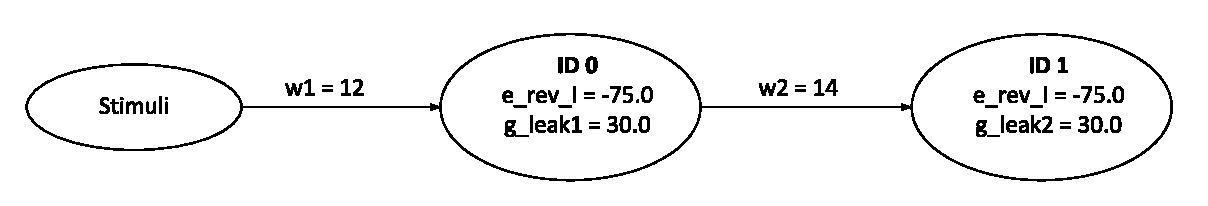
\includegraphics[width=.6\textwidth]{images/topologies/2_neurons_topology.pdf}
	\caption{Network A: a simple system with $2$ sequential neurons and $D=6$ parameters.}
	\label{fig:topology-2neurons}
\end{figure}
\begin{figure}[tb]
	\centering
	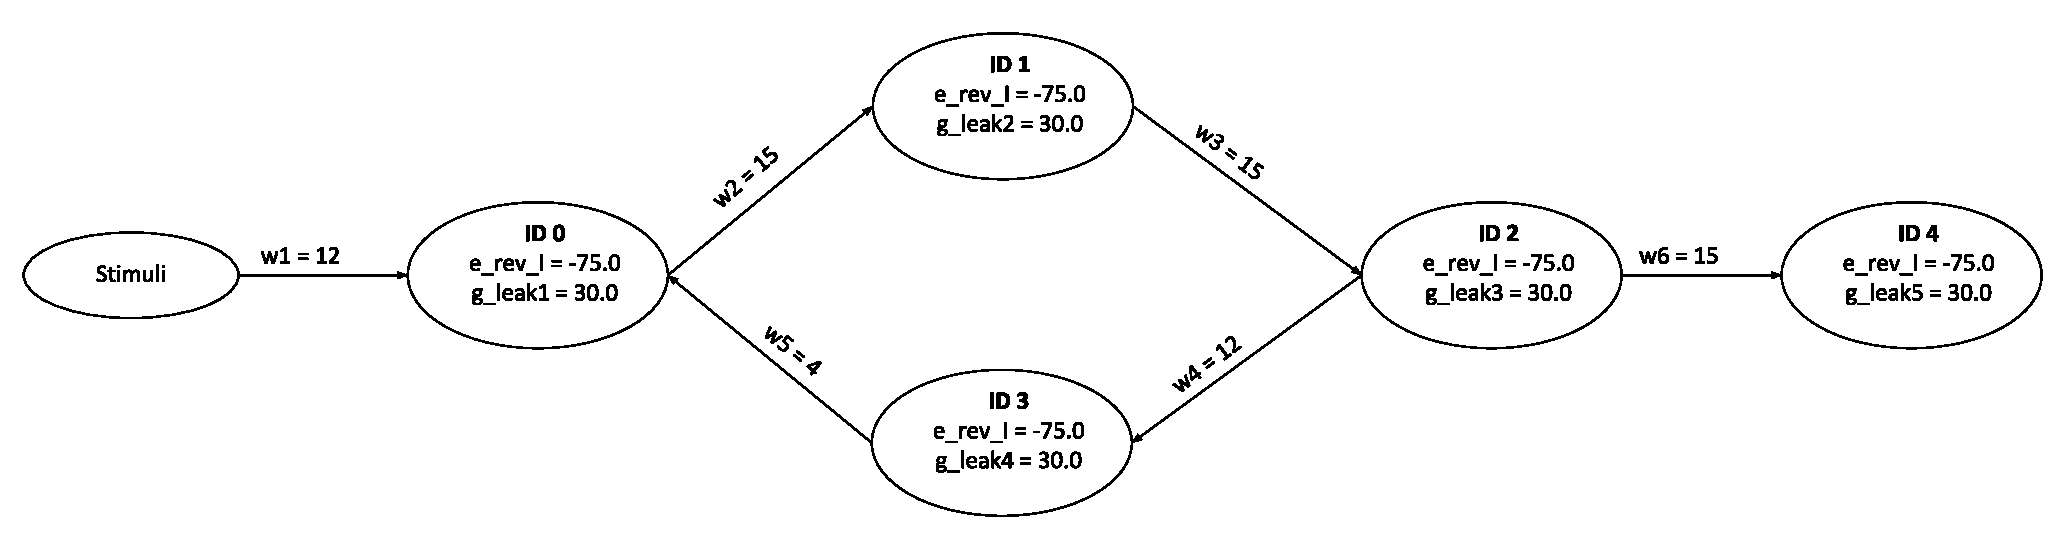
\includegraphics[width=\textwidth]{images/topologies/ring_topology.pdf}
	\caption{Network B: a feedback network with $5$ neurons and $D=12$ parameters.}
	\label{fig:topology-feedback}
\end{figure}
\begin{figure}[tb]
	\centering
	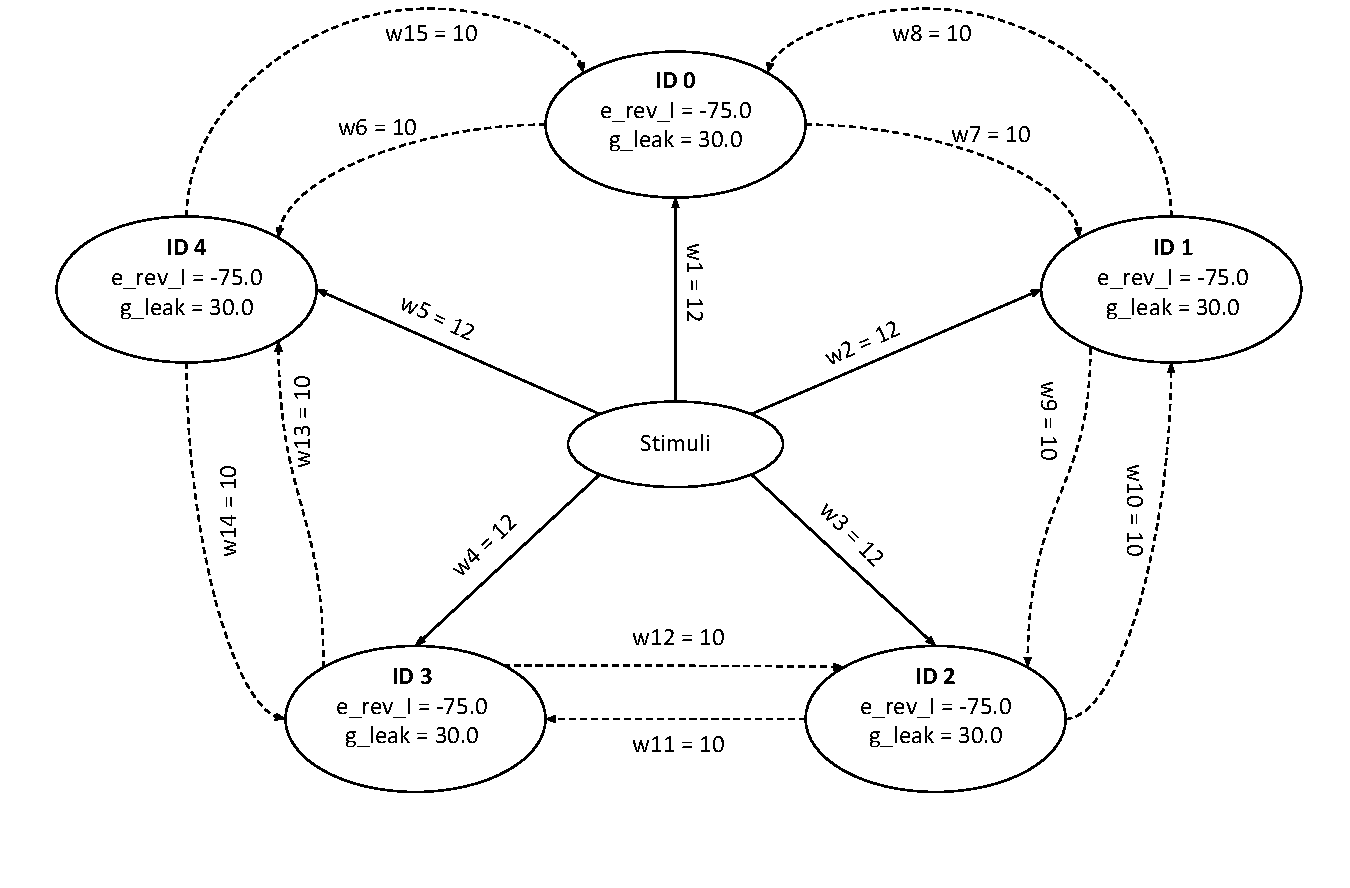
\includegraphics[width=.7\textwidth]{images/topologies/starfish_topology.pdf}
	\caption{Network C: the starfish network with $5$ neurons and $D=17$ parameters. Solid and dashed arcs represent excitatory and inhibitory connections, respectively.}
	\label{fig:topology-starfish}
\end{figure}


%\name{} was implemented using Python 2.7 and the following libraries:  PyNN 0.6, FST-PSO 1.6, numpy 1.14.3, pexpect 4.5, scipy 1.1, and miniful 0.4.
%In all results that follow, the calibration was repeated 30 times to collect statistical information and analyze the average behavior of \name{}.

Figure \ref{fig:target-2neurons} shows the result of the preliminary test on Network A, by comparing the best solution found by \name{} (bottom panel) and the target spiking activity (top panel).
Each dot in the plots represent a spike produced by one of the $2$ neurons in the network (denoted by green and blue colors).
The results show that \name{} correctly estimated  the $6$ parameters and was able to converge to an optimal solution with respect to the spiking activity.
Thus, from a strictly phenomenological point of view, the Spikey chip is reproducing the expected behavior of the target neural network.

\begin{figure}[!ht]
	\centering
	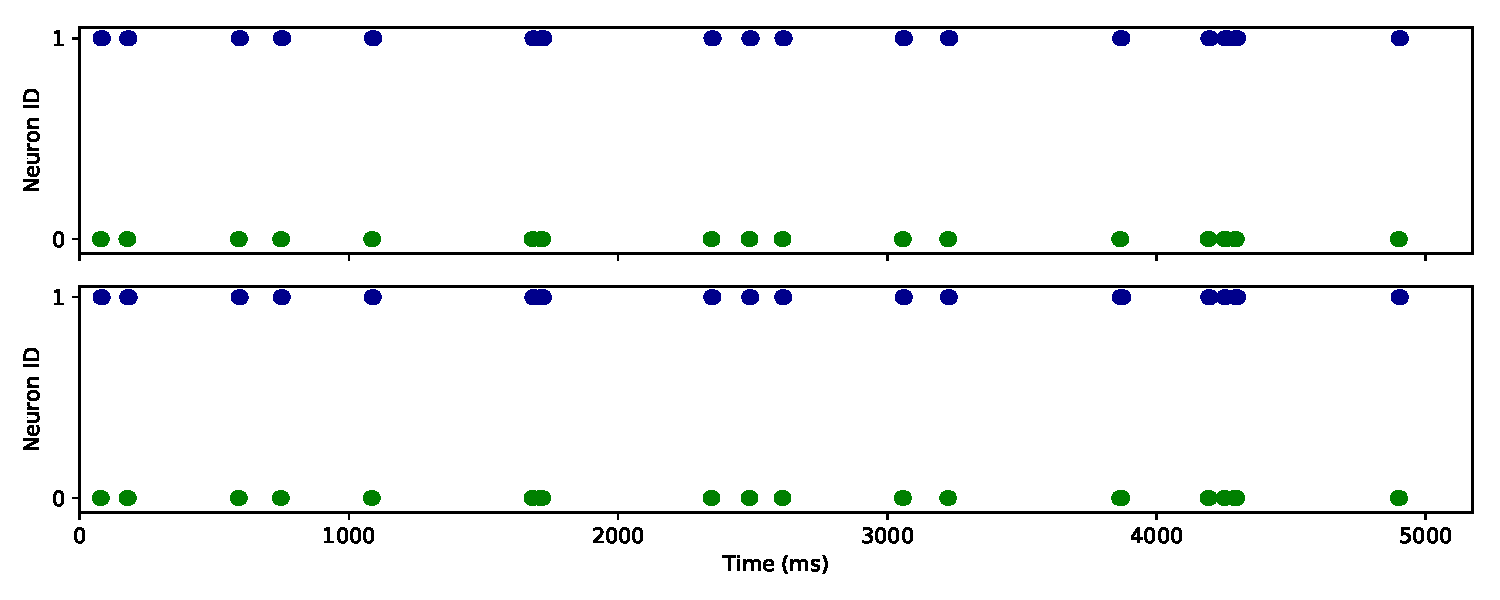
\includegraphics[width=\textwidth]{images/2-neurons-irregular/target_sim.pdf}
	\caption{Comparison of the target (top panel) and the best fitting individual identified by \name{} (bottom panel), in the case of Network A.}
	\label{fig:target-2neurons}
\end{figure}

\todo[inline]{riformulare la caption di Fig.4 (e altre analoghe), non stiamo mostrando il best fitting individual.}
\todo[inline]{MA: Le figure 4 e 5 non si capiscono.  Come si interpretano?}

The six box-plots reported in Figure \ref{fig:boxplots-2neurons} (left side) show the distributions of the optimal parameters identified by \name{} over the $30$ runs.
The red solid lines denote the nominal values used to generate the target data, while the black dashed line represent the best fitting solution found by \name{}. 
Figure \ref{fig:boxplots-2neurons} (right side) shows the convergence plot of FST-PSO.



\begin{figure}[!ht]
	\centering
	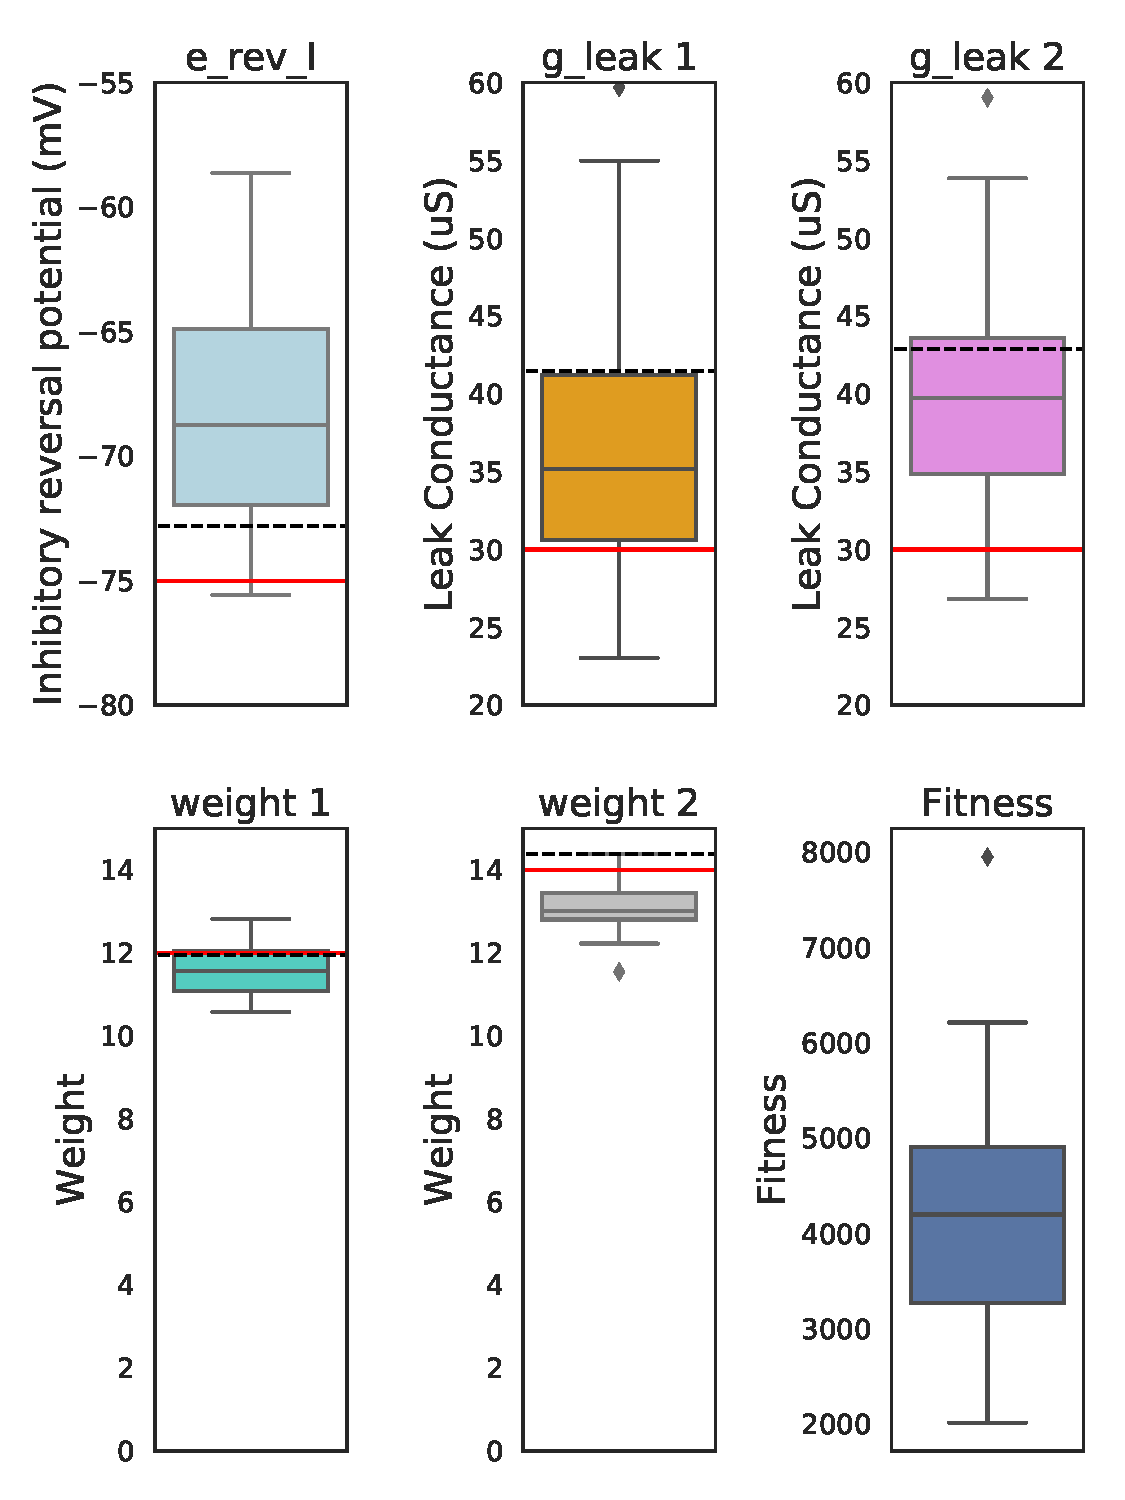
\includegraphics[width=.25\textwidth]{images/2-neurons-irregular/boxplot_best_values-test.pdf}
	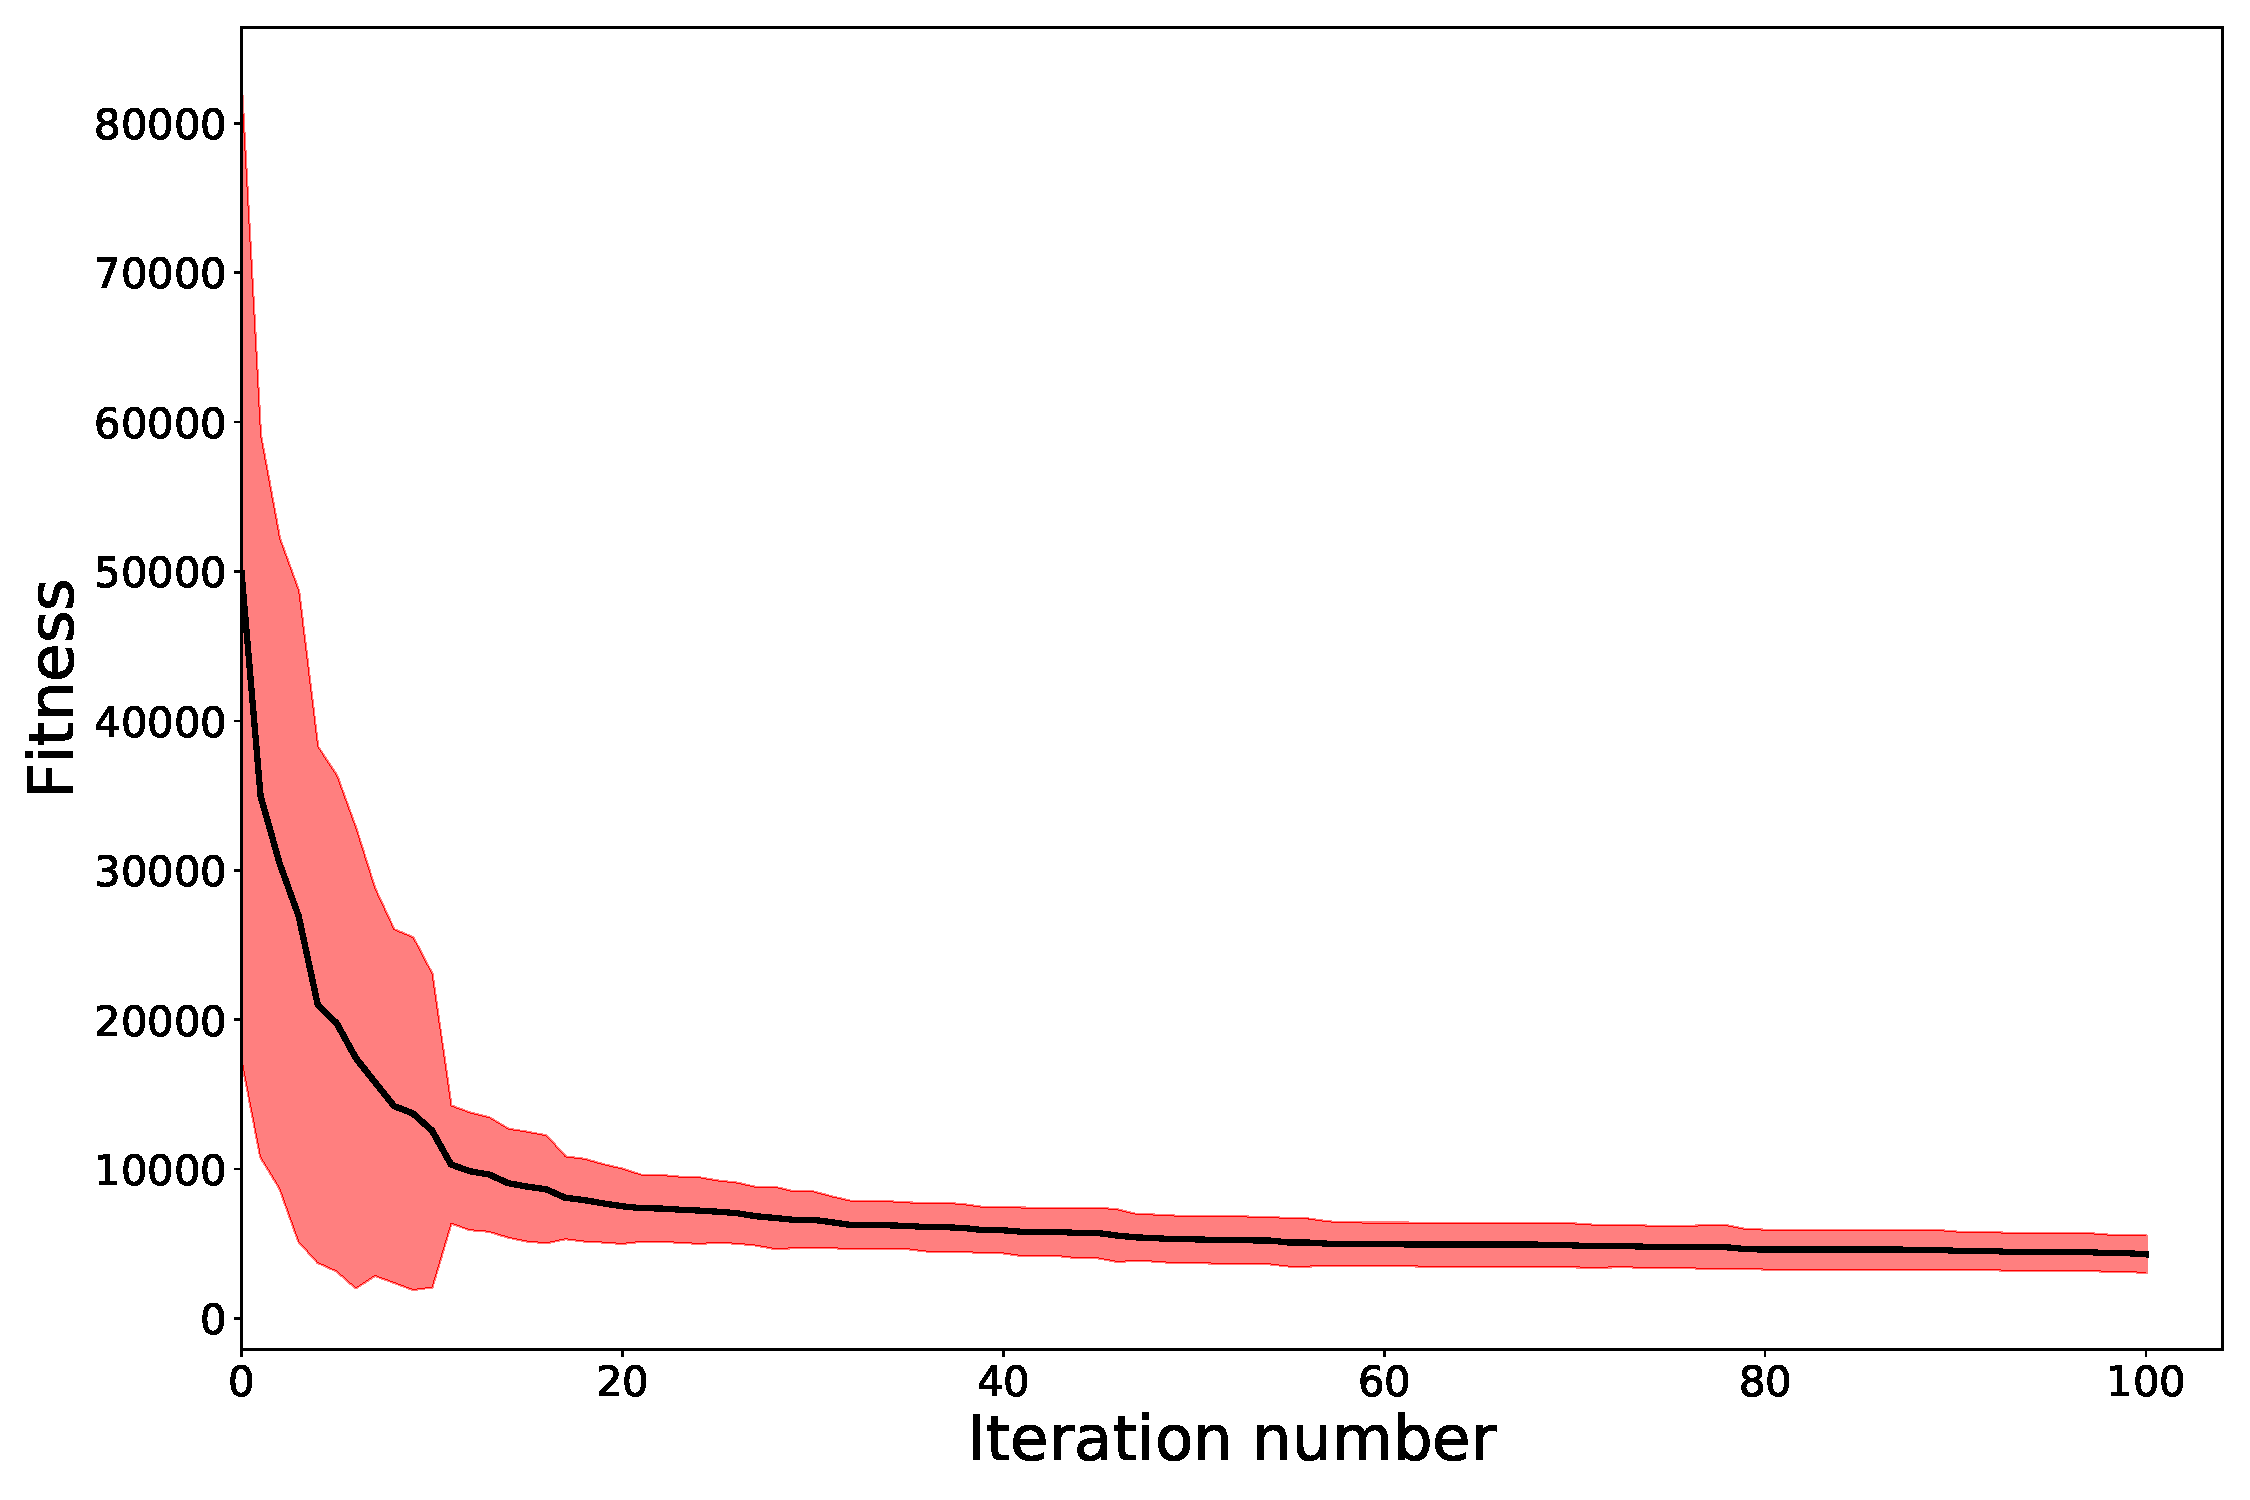
\includegraphics[width=.49\textwidth]{images/2-neurons-irregular/mean.pdf}
	\caption{Results of the calibration of Network A using \name{}. On the left we show the distribution of the optimal parameters. The red solid lines denote the nominal values used to generate the target. The black dashed line denote the best parameterization found by \name{}. On the right we show the convergence plot of FST-PSO. The mean and the standard deviation of the $30$ runs are denoted by the black solid line and the red filled area, respectively.}
	\label{fig:boxplots-2neurons}
\end{figure}

Our results show that multiple parameterizations
\todo[inline]{nel senso che esistono più soluzioni distinte, ma che fittano bene tutte? if so, rifrasare questo "multiple parameterizations"}
are equivalent from the point of view of the spiking activity, that is, they are characterized by a similar fitness value.
It is worth noting that the simulated potentials
\todo[inline]{membrane potentials?}
might differ because of the different parameterization, but this information is lost due to the type of record performed by the chip. 
\todo[inline]{non si capisce una cippa in questa frase}
Again, from the point of view of the pure spiking activity, they
\todo[inline]{they, YOH! ma poi, their di chi?}
dynamics are  completely identical.

We repeated the calibration test Network B, that is, the feedback loop with $5$ neurons and $12$ missing parameters. 
Figure \ref{fig:target-ring} shows that \name{} was again able to perfectly reproduce the expected behavior, fitting all targets with the exception of some exceeding spiking activity mainly at the end of the simulation.
\todo[inline]{nessuna ipotesi sul perché si ottiene questo comportamento?}

\begin{figure}[!ht]
	\centering
	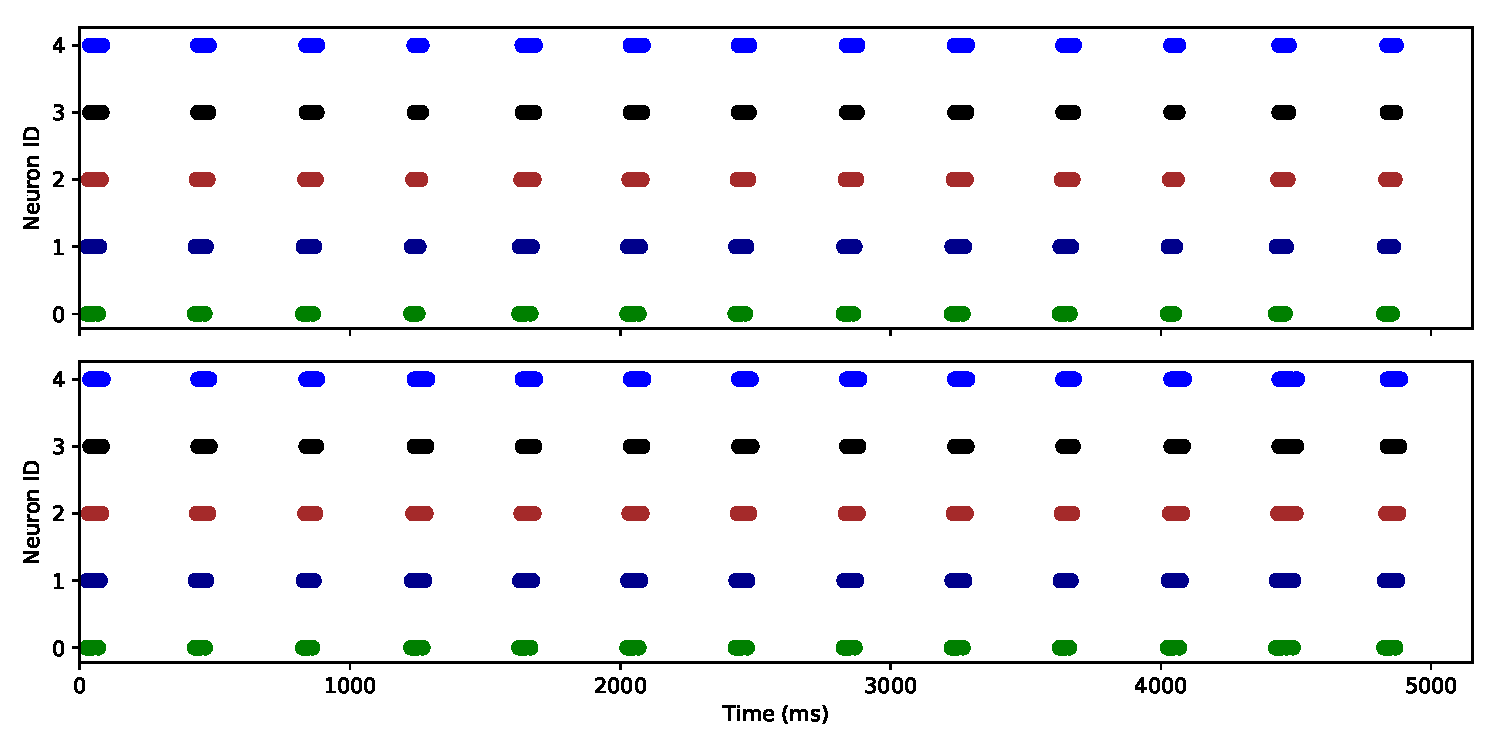
\includegraphics[width=\textwidth]{images/ring-network-regular/target_sim.pdf}
	\caption{Comparison of the target (top panel) and the best fitting individual identified by \name{} (bottom panel), in the case of Network B.}
	\label{fig:target-ring}
\end{figure}

By inspecting the distribution of the $12$ parameters (Figure \ref{fig:convergence-ring}, left side), some values are very different with respect to the nominal values, while some other show a high sensitivity. 
This was actually the case of the weight of neuron $1$: being upstream of the whole network, it requires a high precision to reproduce the correct spiking  activity.
\todo[inline]{eh?}


%\todo[inline]{Daniele, per favore ingrandisci i font dei boxplot. Probabilmente puoi anche dimezzare la larghezza degli stessi. Riguardo le figure delle tracce, puoi drammaticamente ridurre l'altezza delle figure. Nelle figure delle tracce, per quanto riguarda gli ID dei neuroni, per favore solo numeri interi. Togli i titoli nei due panel. Fai anche l'asse delle "x" shared, che tanto è lo stesso sia per target che per simulazione (MSN)}

\begin{figure}[!ht]
	\centering
	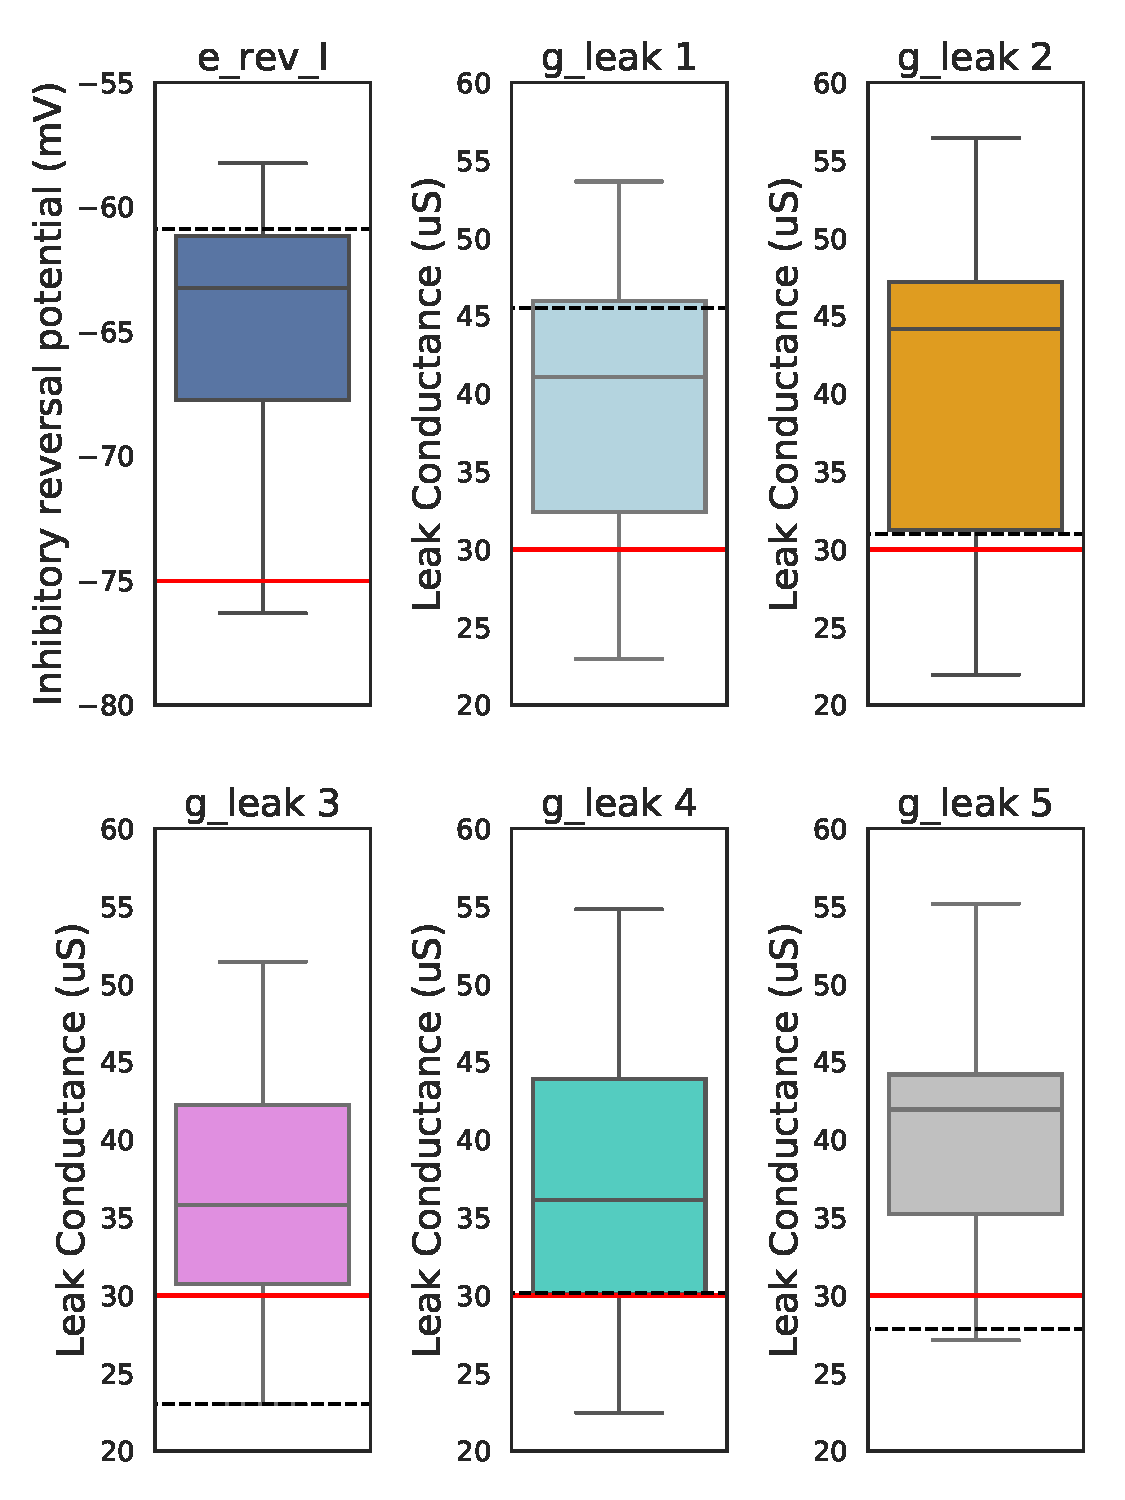
\includegraphics[width=.24\textwidth]{images/ring-network-regular/boxplot-gleak-test.pdf}
	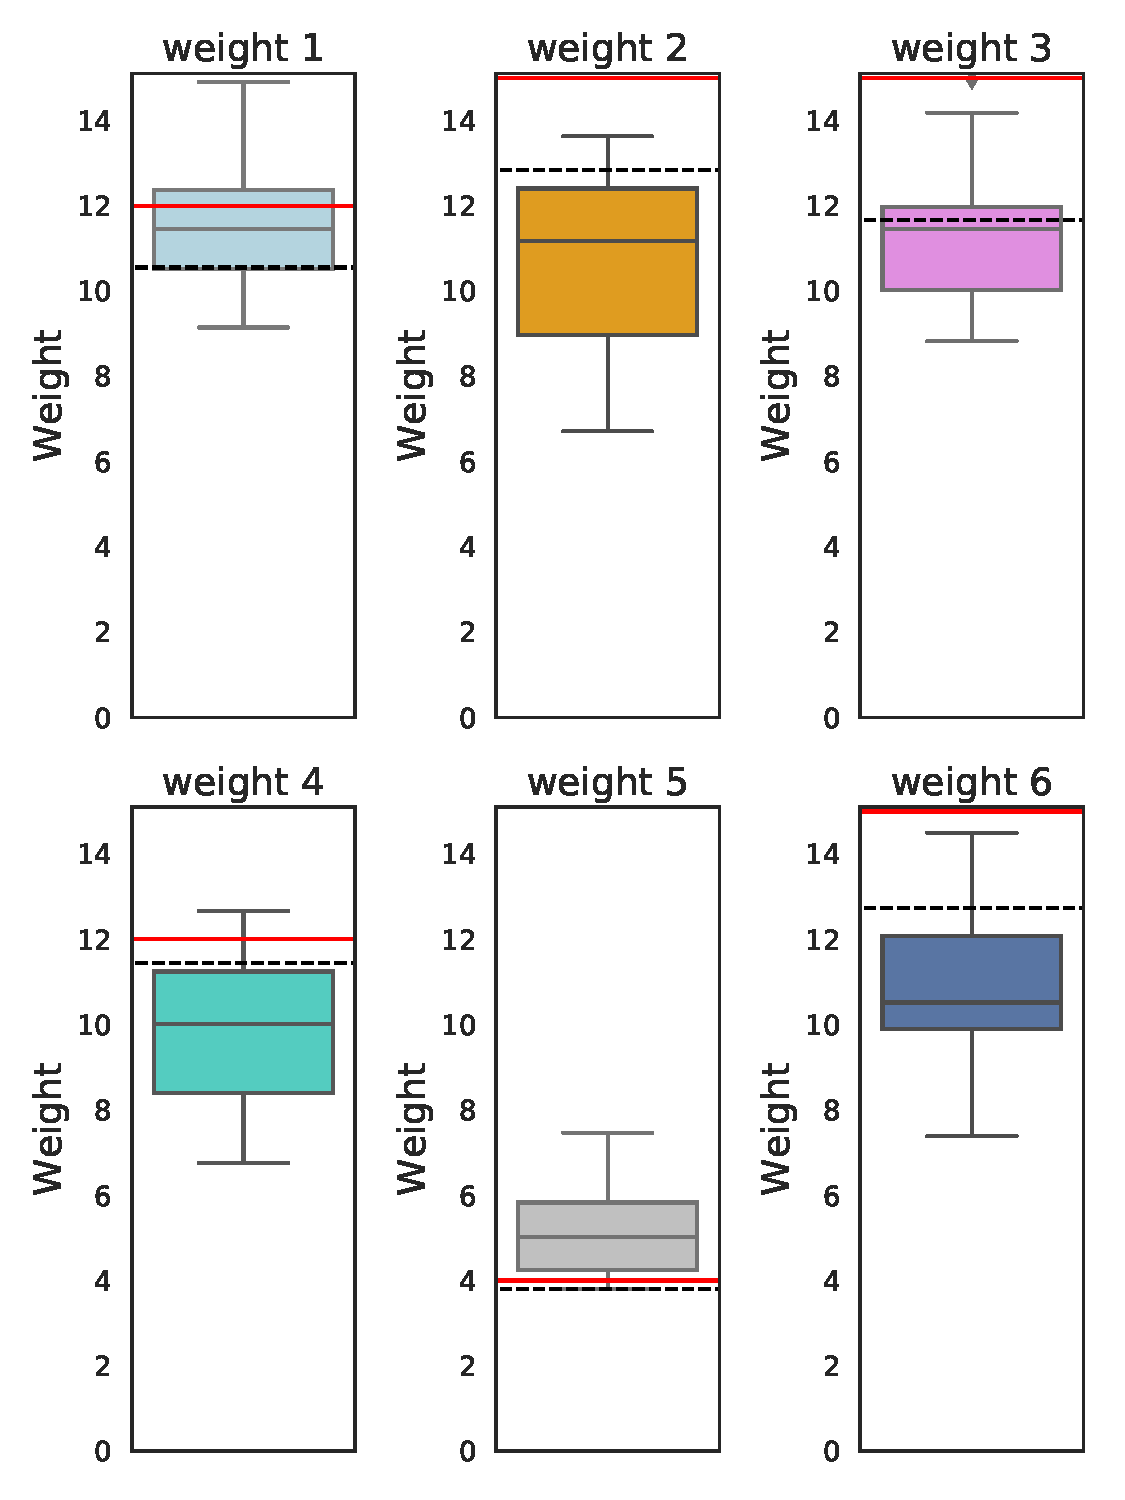
\includegraphics[width=.24\textwidth]{images/ring-network-regular/boxplot-weights-test.pdf}
	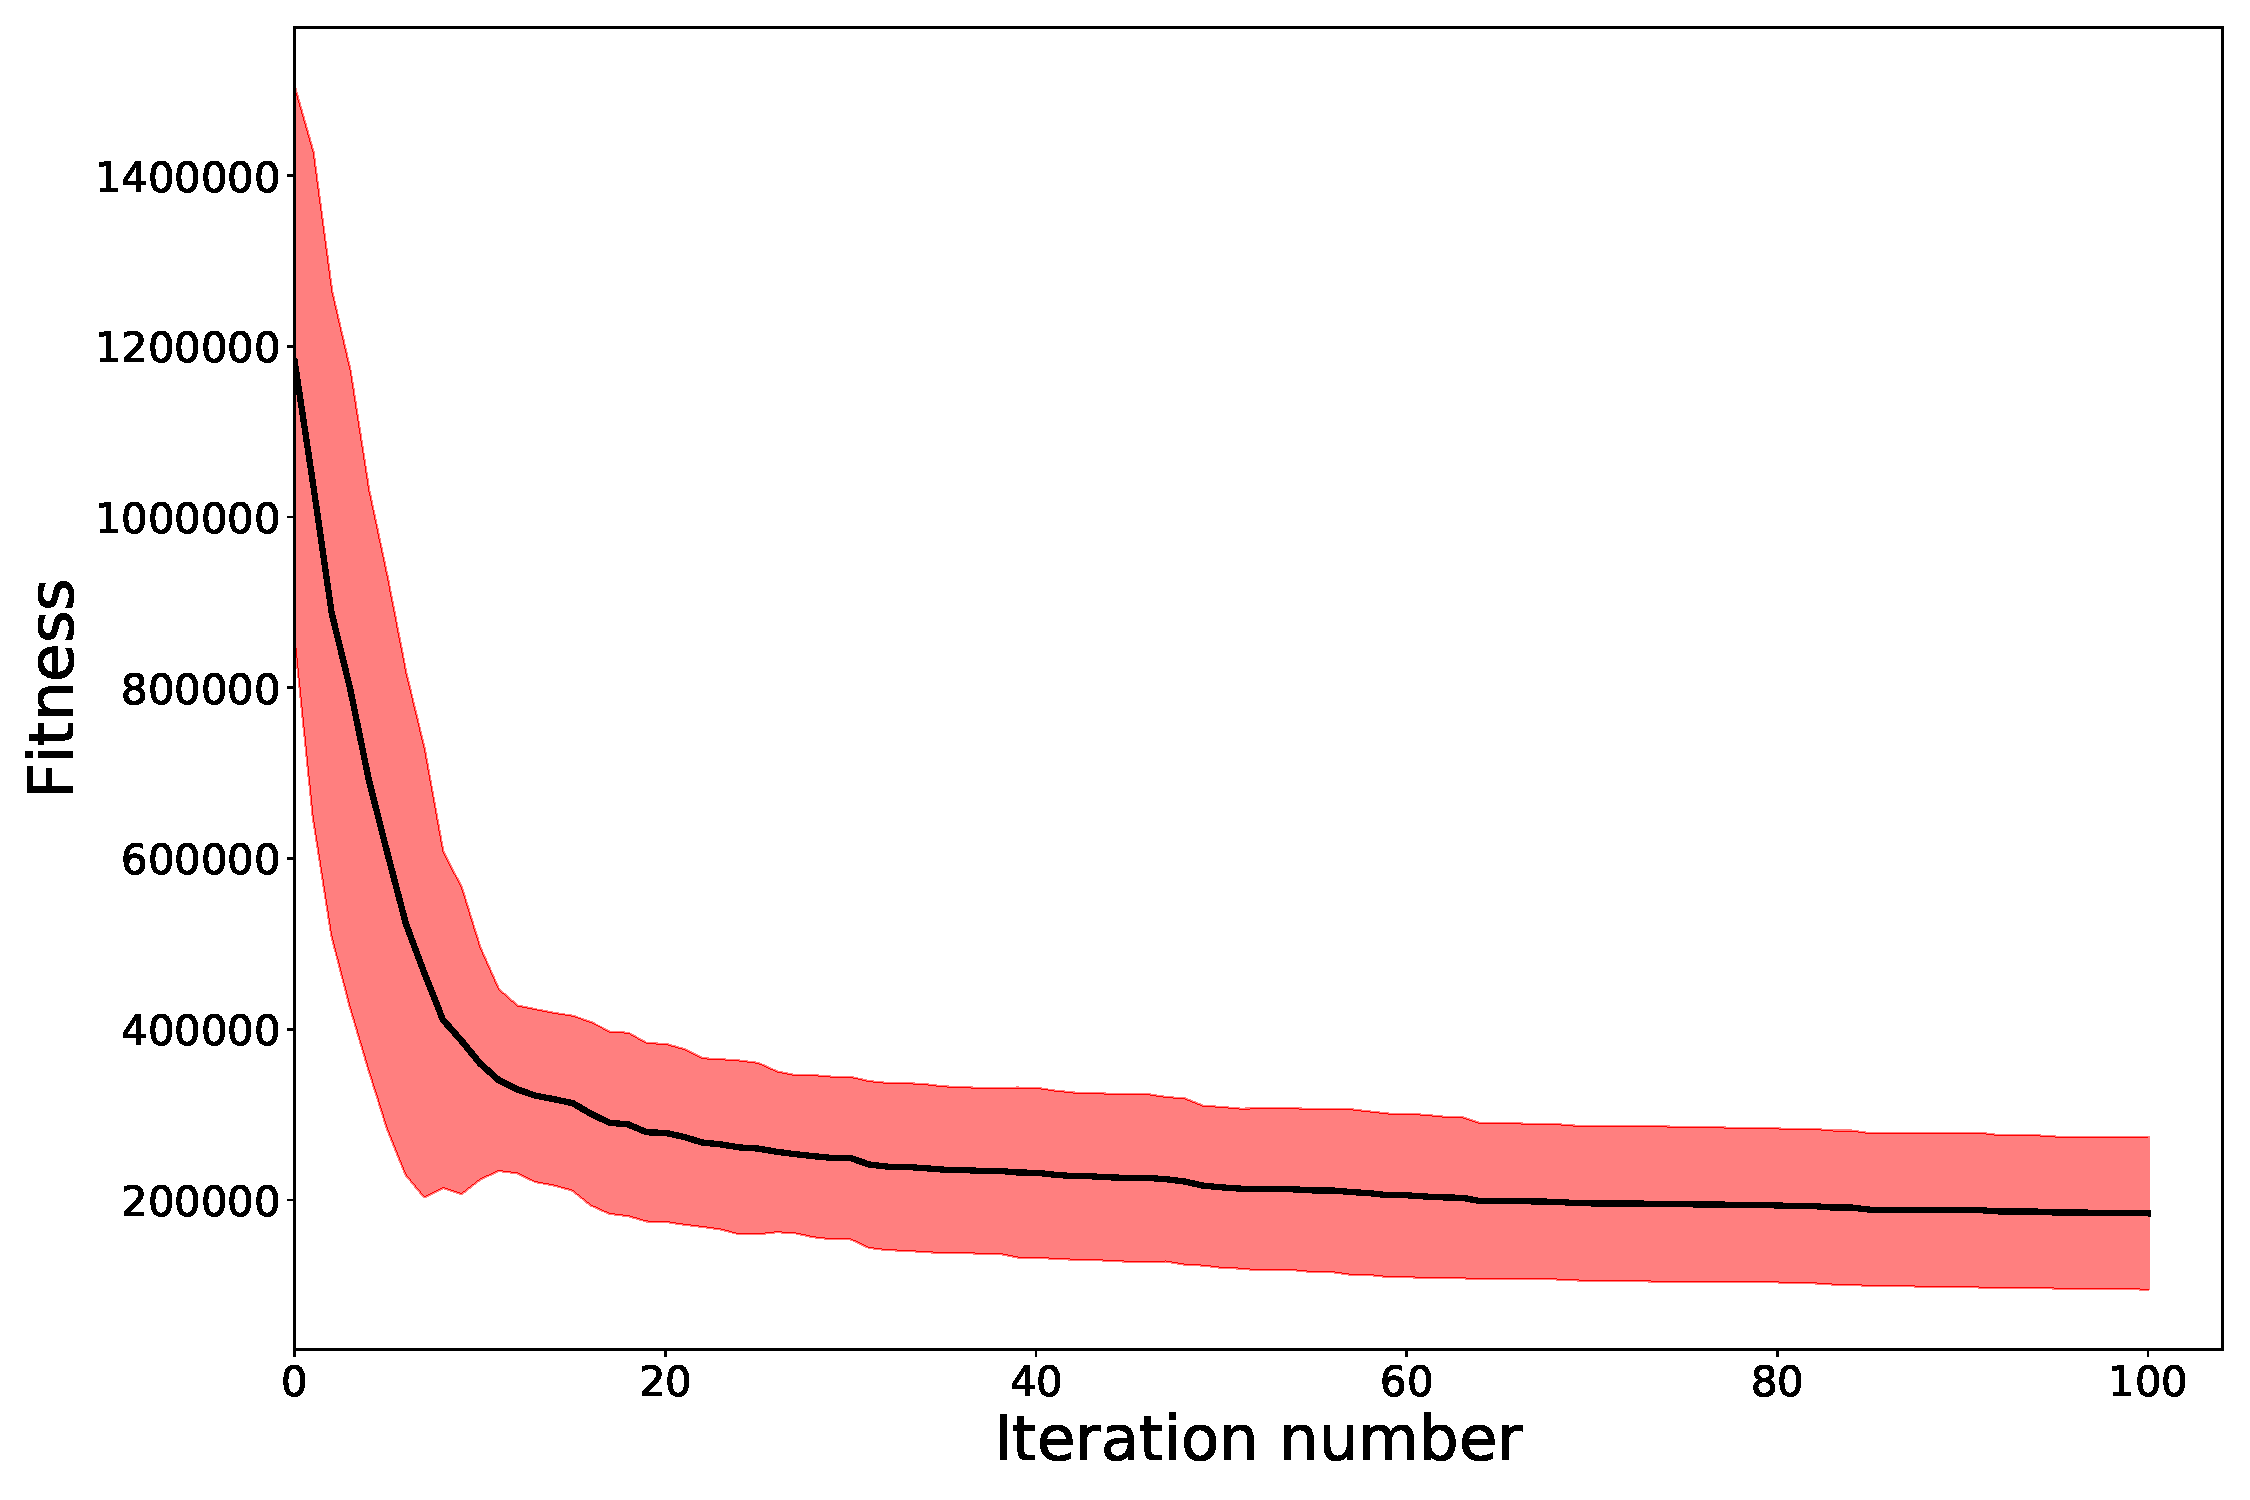
\includegraphics[width=.49\textwidth]{images/ring-network-regular/mean.pdf}
	\caption{Results of the calibration of a Network B using \name{}. On the left we show the distribution of the optimal parameters. The red solid lines denote the nominal values used to generate the target. The black dashed line denote the best parameterization found by \name{}. On the right we show the convergence plot of FST-PSO. The mean and the standard deviation of the $30$ runs are denoted by the black solid line and the red filled area, respectively.}
	\label{fig:convergence-ring}
\end{figure}

In our third group of tests, we calibrated a topology proposed in \cite{suzuki1971dynamics}, corresponding to a simplified model of the starfish nervous system (Network C).
The central nervous system of the starfish is organized as a nerve ring around its mouth, with radial nerves running along the arms.
Although lacking a centralized brain, this system is able to control and coordinate the movements of each arm, and it is considered as one of the earliest and most simple example of nervous system in animals.
%\todo[inline,color=lime]{Simone puoi raccontare qualcosa? (MSN)}
The purpose of this test was to investigate the performance of \name{} in  inferring the weights of inhibitory synapses. 
Figure \ref{fig:topology-starfish} shows the topology of this neural network, where the excitatory and inhibitory connections between the neurons are denoted by solid and dashed lines, respectively.
In this tests, \name{} was not able to identify any solution that perfectly fit with the target data, as shown in Figure \ref{fig:target-stellona}. 
As a matter of fact, the target and simulated spiking sequences differ as the solution found by \name{} is characterized by a slightly different activity (e.g., neuron $4$ spikes two times in the simulation during the interval $0$--$50$ ms, while only a single spike was present in the target).

\begin{figure}[!ht]
	\centering
	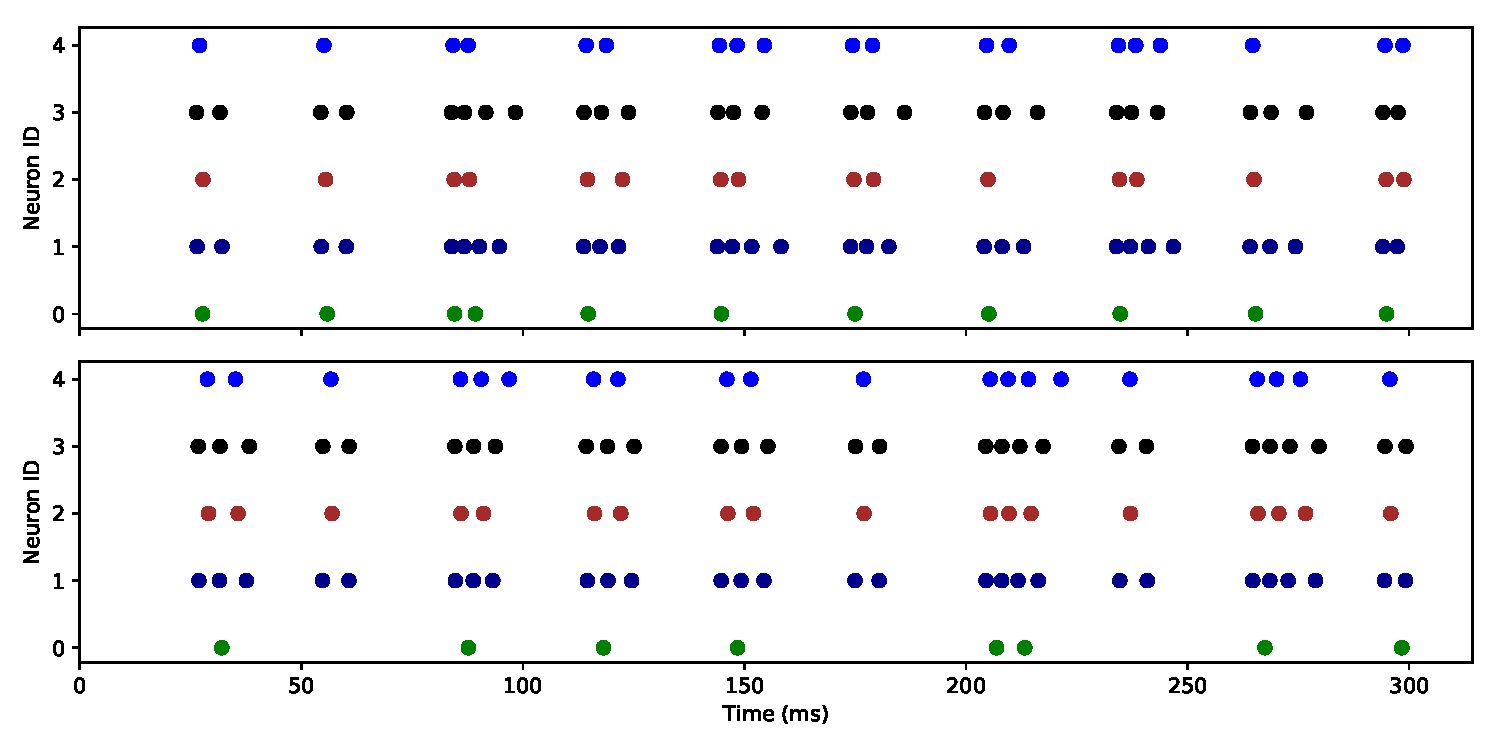
\includegraphics[width=\textwidth]{images/failed-starfish/target_sim.pdf}
	\caption{Comparison of the target (top panel) and the best fitting individual identified by FST-PSO (bottom panel), in the case of Network C. }
	\label{fig:target-stellona}
\end{figure}

We investigated this circumstance in order to determine what was preventing \name{} from a proper convergence to an optimal solution. 
By checking the convergence plots of all runs, we observed that the best global solutions $\textbf{g}$ throughout the 30 runs were actually excellent from the point of view of the fitness value (see Figure \ref{fig:starfishall}); in particular, they were much lower than the fitness values achieved in the experiments previously shown. 
However, many of these solutions were not improved by FST-PSO until the end of the optimization.

\begin{figure}[!ht]
    \centering
    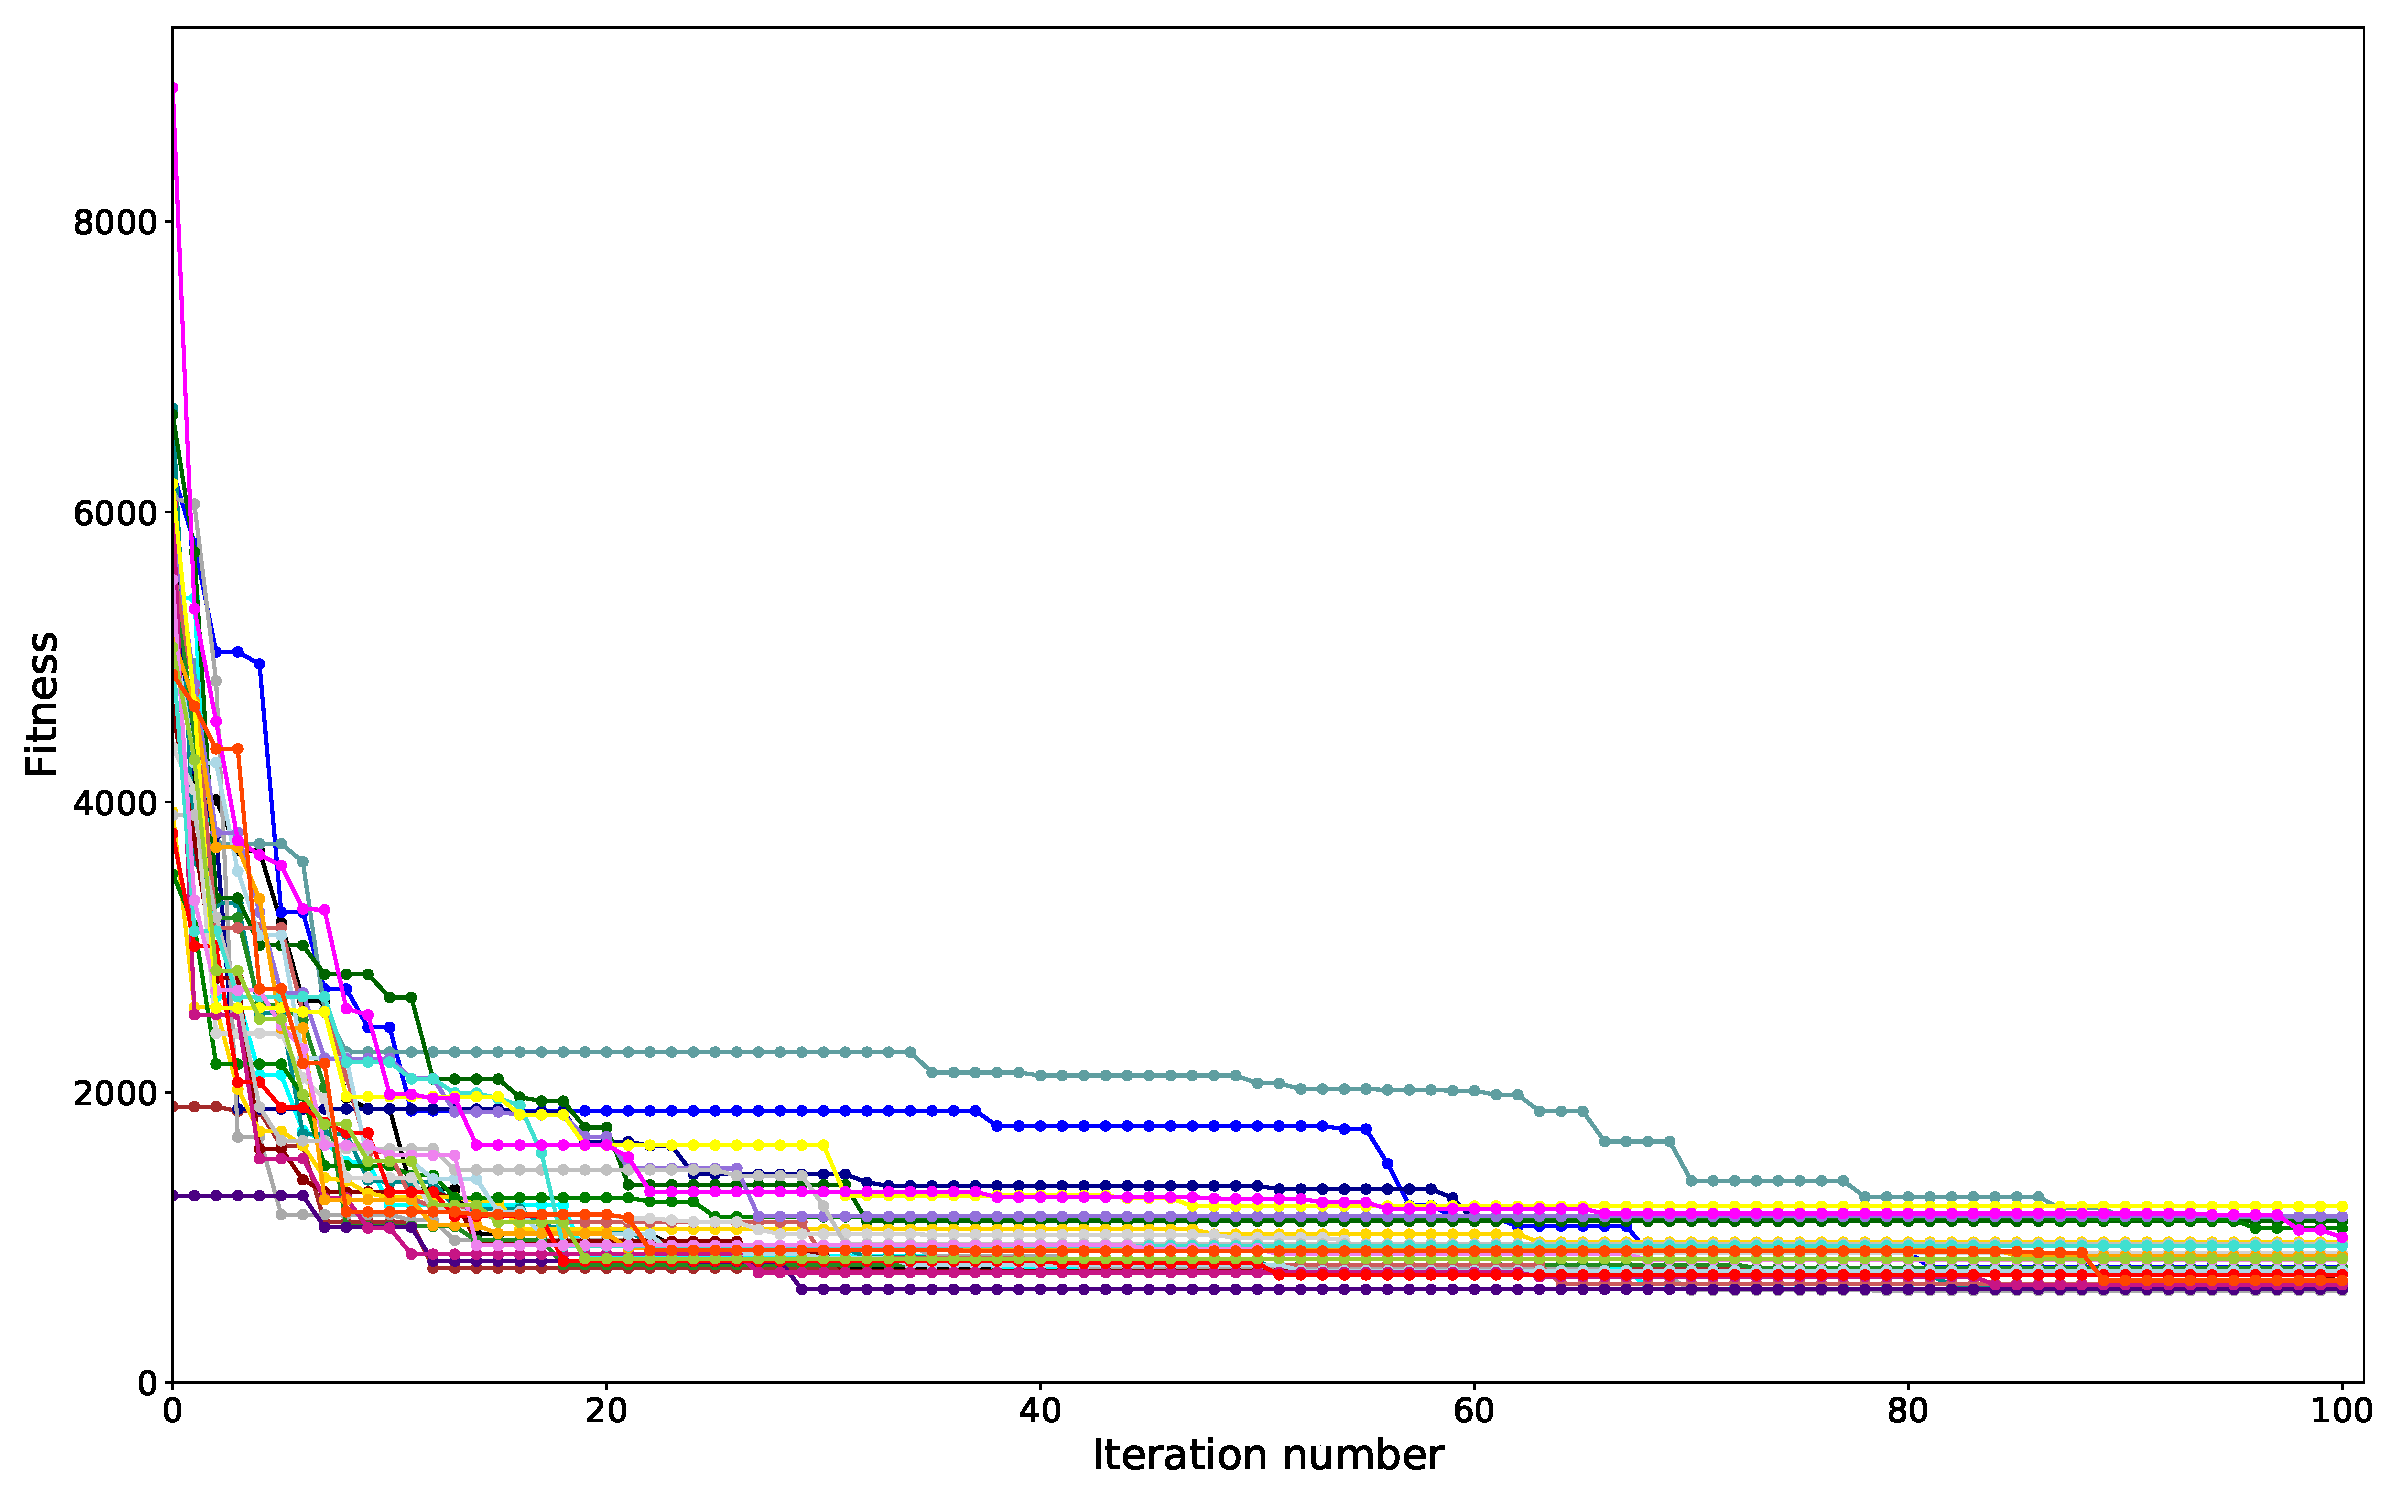
\includegraphics[width=\textwidth]{images/failed-starfish/fitness-each-optimization.pdf}
    \caption{Convergence plots of 30 runs of \name{}. Although many runs seem to immediately converge to an optimal solution, the swarms are actually mislead by wrong evaluations of the fitness value. }
    \label{fig:starfishall}
\end{figure}

\todo[inline]{in caption di fig.9, chiarire "wrong evaluations of the fitness value"}

%\todo[inline]{Papetz, mi rifai figura 9 in maniera piu comprensibile? togli pure la legenda che non è molto informativa e ingrandiscimi i font sugli assi pls (MSN)}


By simulating such solutions,
\todo[inline]{dai cazzo}
we realized that the fitness values of $\textbf{g}$ calculated by \name{} were actually wrong: the values calculated \emph{a posteriori}  were much higher due to a very poor fitting with respect to the target traces.
\todo[inline]{non si capisce niente... cosa vuol dire che erano sbagliate? ma non si può scrivere una cosa del genere in un paper!}
By repeating the simulations several times
\todo[inline]{magari specificare nelle stesse condizioni, eh}
we noted that, in a few occasions,  Spikey was producing simulated traces that were different
\todo[inline]{diverse da cosa?}
and more similar to the target behavior.
This stochasticity
\todo[inline]{non capisco, a me questa (nella sequenza di spike ottenuta) sembra una stocasticità a posteriori, questa frase per me non ha senso (o non si capisce cosa volevate dire); oltretutto, all'inizio del paper si parla di noise dovuto ad altro, quindi qui il lettore resta confuso (e io pure)}
introduces  sudden, unpredictable and misleading modifications of the spiking activity, which in turn can lead to wrong evaluations of the fitness value.
\todo[inline]{gate sparire qualsiasi wrong da questo paper}
Hence, the best particles $\textbf{g}$, 
\todo[inline]{perché plurale?}
characterized by an excellent fitness values that do not reflect the quality of their own parameterizations---are actually driving the swarms into wrong areas of the search space.
Fatally, the swarm is no longer able to escape that region and \name{} eventually outputs poor
\todo[inline]{poor no, cambiare aggettivo}
parameterizations associated to excellent fitness values.
\todo[inline]{tutto questo mi fa pensare che ci sia un problema nella definizione della fitness ;) il revisore ci stronca se descriviamo/discutiamo i risultati in questo modo (e fa bene)}


\section{Discussion}
\label{sec:discussion}
Spikey's  stochasticity
\todo[inline]{idem come sopra}
implies that two independent simulations of the same model, performed using the same parameterization, yield different spiking traces.
We discuss this behavior, and its implications, by performing 1000 simulations of the starfish model. 
Figure \ref{fig:distributionfiring} show the strip plots of the spiking events of the five neurons. 


\begin{figure}[!ht]
    \centering
    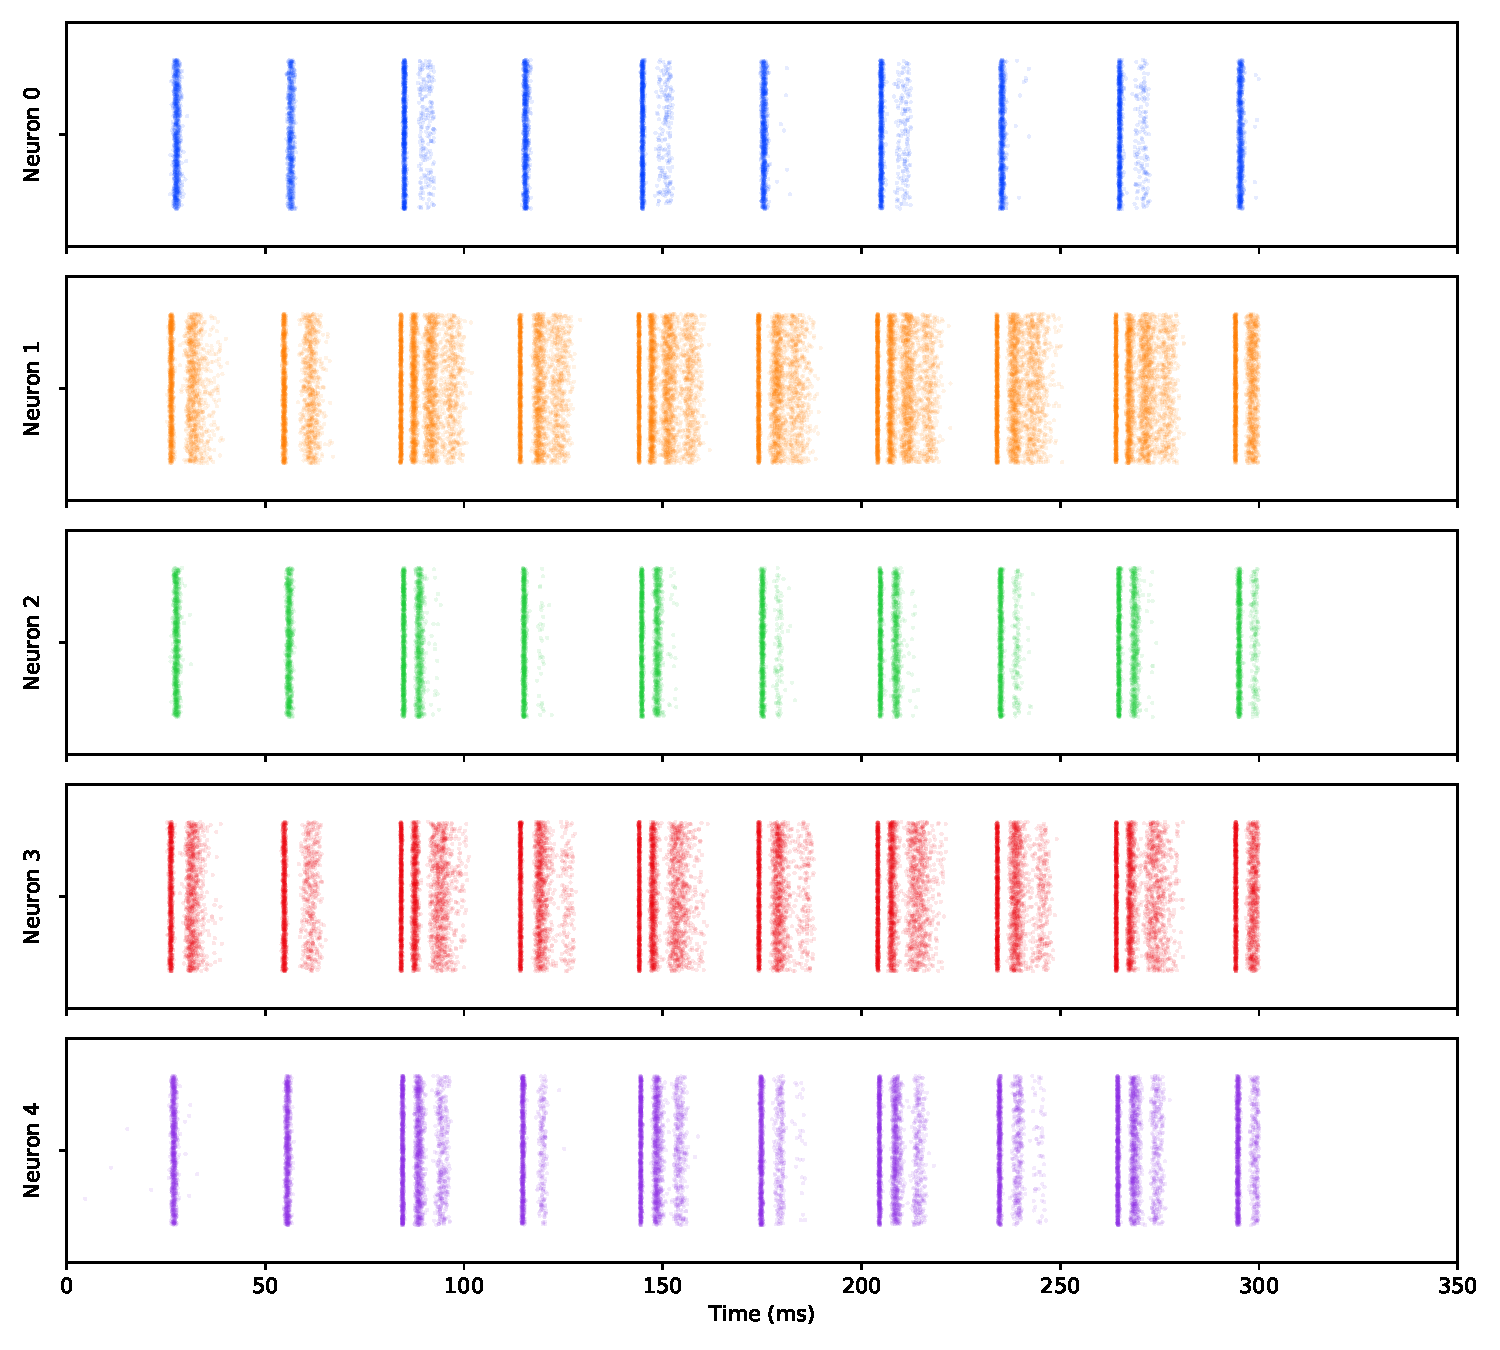
\includegraphics[width=\textwidth]{images/failed-starfish/distribution-firing-light.pdf}
    \caption{1000 simulated traces of the spiking activity of the five neurons in the starfish network. All simulations were performed using the same parameterization. A darker color corresponds to a higher probability of a spiking event. The scattering and misalignment of points highlight the stochasticity of Spikey's simulation.}
    \label{fig:distributionfiring}
\end{figure}

Thanks to alpha blending, the darker areas correspond to a higher probability of a spiking event at that specific time point---a fully deterministic simulation would produce perfectly dark vertical single-pixel bars.
On the contrary, the traces show that the spikes are shattered
\todo[inline]{scattered?}
in time, and many lighter areas confirm that different simulations can yield radically different outcomes, corresponding to radically different fitness values.
One striking example is the trace for Neuron 3: every simulation basically produces a different outcome, affecting the fitness values at each repetition. 
In particular, if one of those ``outlier'' simulations perfectly fits with the target behavior, that will correspond to a very low fitness value that will hardly be repeated by the following attempts in that region of the search space. 
\todo[inline]{riscrivere ultima frase, pls (e aggiustare tempi verbali)}

The issue we just described represents the main limitation to the application of \name{} for the automatic calibration of NCs like Spikey, which is characterized by a stochastic behavior due to physical aspects. 
As future developments, we will investigate a novel fitness function able to mitigate this problem, even though this task is far from trivial.
\todo[inline]{riformulare}
As a matter of fact, Spikey's simulation produces a peculiar trace composed of a list of spiking events, which are temporally misaligned and whose count
\todo[inline]{count?}
can differ across multiple simulations. 
Due to this circumstance, it is impossible to calculate an ``average'' trace out of multiple simulations.
\todo[inline]{e a cosa servirebbe?}
As an alternative we could, in principle, assess the fitness evaluations by ``binning'' the traces, in order to calculate the histograms of spiking probabilities.
Then, we could use fixed thresholds to determine whether the putative parameterization actually yields a spiking event in that region with a high probability. 
\todo[inline]{supercazzole a gogo... provare a riformulare in modo che anche un essere umano medio possa capire?}
In the latter case, the goal of the calibration could be restated as an expectation maximization, that is, FST-PSO
\todo[inline]{SNATCH?}
would be used to maximize the likelihood of experimental data given the putative parameterization.

As soon as we will define a sound fitness function for this calibration problem, we will increase the size of the neural network,
\todo[inline]{ragazzi, perché tirarsi la merda addosso da soli? riscrivere pls}
ultimately aiming at the modeling of biologically meaningful topologies---like the sensory networks of model insects  \cite{namiki2009reconstruction,Pfeil2013}---in order to use \name{} to calibrate the system and reproduce their peculiar spiking behavior.
\todo[inline]{MA: concordo con il commento sopra.  La descrizione del lavoro sembra essere: \emph{abbiamo provato a fare due cose e non hanno funzionato; inoltre non sappiamo bene perch\`{e}}.  Ad un certo punto si era anceh detto di provare pi\`{u} simlazioni dell'architettura "star"; non si capisce bene se ci\`{o} sia stato fatto o no.\\Direi che cos\`{i} il papero non funziona molto.}

\section*{Author Contributions}
MSN and DMP contributed conception and design of the study; DMP and MSN implemented SNATCH; SS provided biological domain knowledge; DMP performed the statistical analysis; DMP, MSN, SS, PC and DB analyzed the results; DMP and MSN wrote the first draft of the manuscript; MA launched the research project as part of the activitities of the University of Milan-Bicocca NeuroMI Centre. MA, SS, PC and DB contributed to the writing of the manuscript. All authors contributed to manuscript revision, read and approved the submitted version.

\section*{Funding}
Details of all funding sources should be provided, including grant numbers if applicable. Please ensure to add all necessary funding information, as after publication this is no longer possible.

\section*{Acknowledgments}
We want to acknowledge the Universit\"at Heidelberg for kindly granting us access to the prototype of the Spikey neuromorphic chip.


\section*{Data Availability Statement}
The datasets [GENERATED/ANALYZED] for this study can be found in the [NAME OF REPOSITORY] [LINK].
% Please see the availability of data guidelines for more information, at https://www.frontiersin.org/about/author-guidelines#AvailabilityofData

\todo[inline]{la biblio è da sistemare}

\bibliographystyle{frontiersinSCNS_ENG_HUMS} % for Science, Engineering and Humanities and Social Sciences articles, for Humanities and Social Sciences articles please include page numbers in the in-text citations
% \bibliographystyle{frontiersinHLTH&FPHY} % for Health, Physics and Mathematics articles
\bibliography{neuretti}

%%% Make sure to upload the bib file along with the tex file and PDF
%%% Please see the test.bib file for some examples of references

\end{document}
